\chapter{Controle Bancário: Versão 1}\label{bancario}

Neste  capítulo, será  apresentado  o processo  de  desenvolvimento da  primeira
versão  da aplicação {\bf  ControleBancario}. Trata-se  uma aplicação  de gestão
bancária cujo modelo de entidades é apresentado na Figura~\ref{figUML}.

\vspace{0.2cm}

O primeiro passo é  a criação de um projeto através da  execução, em um terminal
ou  através  da utilização  de  algum IDE,  do  comando  {\bf grails  create-app
  ControleBancario}\footnote{Para  obter a  lista completa  de  comandos Grails,
  executar o comando {\bf grails help} em um terminal.}.  \index{Comandos!grails
  create-app}  No  caso do  Intellij  IDE,  a criação  de  um  projeto segue  os
seguintes passos: 

\vspace{0.2cm}

\begin{itemize}

\item No  menu principal, selecione: {\bf Create  New Project} $\Longrightarrow$
  {\bf Grails}.  

\vspace{0.2cm}

\item Em nome do projeto, digite {\bf ControleBancario} e clique em {\bf Finish}
  (Figura~\ref{criaProjFig}).   O Intellij  IDE  executa o  comando {\bf  grails
  create-app}. 

\end{itemize}

\begin{figure}[htbp]
\centering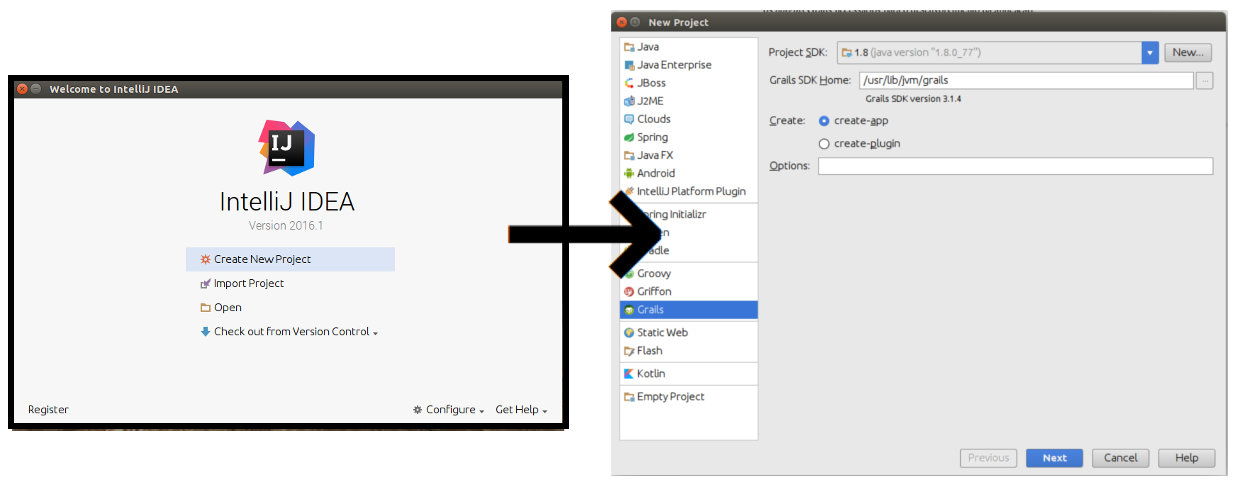
\includegraphics[width=14cm]{IDE}
\caption{Criação do Projeto ControleBancario.}
\label{criaProjFig}
\end{figure}

Caso  esses  passos  sejam  realizados  com  sucesso,  o  projeto  da  aplicação
(hierarquia  de diretórios) está  criado.  Ou  seja, foi  criado um  conjunto de
arquivos  e diretórios para  o projeto.  Essa hierarquia  de diretórios  segue o
paradigma  {\it Convention  Over  Configuration}.  Ou  seja, os  desenvolvedores
seguem  as convenções  e já  sabem {\it  a priori}  onde se  encontram  todos os
elementos  que compõem  a aplicação  em desenvolvimento.   Um {\it  overview} do
conteúdo   desses   diretórios    é   apresentado   na   Tabela~\ref{grailsTbl}.
\index{Convenção!{\it versus}~Configuração}

\vspace{0.5cm}

\begin{table}[htbp]
\centering
\begin{tabular}{p{4.5cm} | p{9cm}}

\toprule 
\rowcolor{Gray} 

\textbf{Diretório} & \textbf{Descrição}\\ 
\midrule
{\bf  grails-app/domain} &  Onde  se  encontra o  M  do MVC.  Ou  seja, onde  se
encontram as classes de Domínio, ou modelos.  \\ 
\midrule
{\bf grail-app/controllers}  & Onde se  encontra o C  do MVC.  Ou seja,  onde se
encontram os controladores.  \\ 
\midrule
{\bf  grails-app/views} &  Onde  se  encontra o  V  do MVC.   Ou  seja, onde  se
encontram as visões (arquivos.gsp – Groovy Server Pages). \\ 
\midrule
{\bf  grails-app/taglib} &  Onde se  encontram  as bibliotecas  de marcas  ({\it
  taglibs}) criadas pelo usuário. \\ 
\midrule
{\bf grails-app/services} & Onde se encontram as classes utilizadas na camada de
serviços (serviços web). \\ 
\midrule 
{\bf  grails-app/i18n}   &  Onde  se   encontram  os  arquivos   relacionados  à
internacionalização.  \\ 
\midrule
{\bf grails-app/conf}  & Onde se  encontram as configurações da  aplicação, tais
como a configuração do banco (application.yml), entre outros. \\ 
\midrule
{\bf grails-app/init} & Onde se  encontra a classe BootStrap.groovy utilizada na
inicialização de dados da aplicação, entre outros. \\ 
\midrule
{\bf grails-app/assets}  & Esse diretório possui três  diretórios ({\it images},
{\it  javascript}  e  {\it  stylesheets})  onde se  encontram  os  {\it  assets}
utilizados na aplicação. \\ 
\midrule
{\bf src/main/groovy}  & Onde se  encontram outros códigos-fonte Java  ou Groovy
que não são modelos, controladores, visões ou serviços. \\ 
\midrule   
{\bf src/test/groovy} & Onde se encontram os testes unitários da aplicação.  \\ 
\midrule
{\bf src/integration-test/groovy} & Onde se encontram os testes de integração da
aplicação.  \\ 
\bottomrule
\end{tabular}
\caption{Projeto Grails: {\it Overview} dos Diretórios.}
\label{grailsTbl}
\end{table}

\newpage

\section{Configuração da aplicação} 

\vspace{0.5cm}

Considerando  que  o  projeto  foi  criado,  o próximo  passo  é  configurar  as
dependências   e  instalar   os  {\it   plugins}  Grails   necessários   para  o
desenvolvimento da aplicação.  

\subsection{Instalação     de      {\it     plugins}     e      definição     de
  dependências}\label{secPlugins}

\vspace{0.5cm}

Na  implementação  das  funcionalidades  da  aplicação  {\bf  ControleBancario},
discutidas nesse  capítulo, será utilizado  o plugin Grails  {\bf br-validation}
que auxilia a validação de campos CPF, CNPJ e CEP das entidades da aplicação. 

\vspace{0.5cm}

Desde  a versão  3 do  Grails, a  inserção de  dependências de  {\it  plugins} é
realizada no arquivo {\bf build.gradle}. O conteúdo desse arquivo, relacionado à
configuração   de   dependências   de    {\it   plugins},   é   apresentado   no
Código~\ref{codBuildGradle}.  Dessa forma, para instalar  o plugin {\bf
  br-validation}        adicione         o        comando        \texttt{compile
  "org.grails.plugins:br-validation:0.3"}, descrevendo a dependência, no arquivo
{\bf     build.graddle}    conforme     apresentado    na     linha     13    do
Código~\ref{codBuildGradle}.
  
\index{Comandos!grails install-plugin} 
\index{Plugins!br-validation}

\vspace{0.5cm}

\begin{lstlisting}[numbers=left,  caption={\bf  build.gradle}  (configuração  de
    {\em plugins}), frame = trBL, float=htbp, label=codBuildGradle, basicstyle =
    \footnotesize] 
dependencies {
    compile "org.springframework.boot:spring-boot-starter-logging"
    compile "org.springframework.boot:spring-boot-autoconfigure"
    compile "org.grails:grails-core"
    compile "org.springframework.boot:spring-boot-starter-actuator"
    compile "org.springframework.boot:spring-boot-starter-tomcat"
    compile "org.grails:grails-dependencies"
    compile "org.grails:grails-web-boot"
    compile "org.grails.plugins:cache"
    compile "org.grails.plugins:scaffolding"
    compile "org.grails.plugins:hibernate4"
    compile "org.hibernate:hibernate-ehcache"
    compile "org.grails.plugins:br-validation:0.3"
    console "org.grails:grails-console"
    profile "org.grails.profiles:web:3.1.4"
    runtime "org.grails.plugins:asset-pipeline"
    runtime "com.h2database:h2"
    runtime "org.postgresql:postgresql:9.3-1101-jdbc41"
    testCompile "org.grails:grails-plugin-testing"
    testCompile "org.grails.plugins:geb"
    testRuntime "org.seleniumhq.selenium:selenium-htmlunit-driver:2.47.1"
    testRuntime "net.sourceforge.htmlunit:htmlunit:2.18"
}
\end{lstlisting}

\newpage

\subsection{Configuração do banco de dados}\index{Banco~de~Dados}

\vspace{0.2cm}

O SGBD H2, provido pelo Grails,  é adequado para aplicações de demonstração, mas
em algum  momento os  desenvolvedores precisarão de  um SGBD mais  robusto, tais
como  {\bf  MySQL},  {\bf  Postgresql}  ou  {\bf  Oracle}.   Com  propósitos  de
ilustração, o SGBD {\bf Postgresql} será utilizado na implementação da aplicação
{\bf ControleBancario}. No entanto, o leitor pode usar outro SGBD relacional.

\vspace{0.2cm}

Para o uso de outro SGBD, tais  como {\bf MySQL} ou {\bf Oracle}, os passos para
suas  configurações são  análogos aos  apresentados a  seguir para  o  SGBD {\bf
  Postgresql}: 

\vspace{0.2cm}

\begin{itemize}

\item  Habilite  o  driver  {\it   JDBC}  do  SGBD  {\bf  Postgresql},  conforme
  apresentado na linha 18 do Código~\ref{codBuildGradle}; e 

\vspace{0.3cm}

\item Altere o arquivo {\bf grails-app/conf/application.yml} para configurar o
  acesso ({\it driver}, {\it url}, {\it  username} e {\it password}) ao banco de
  dados.   O conteúdo  desse arquivo,  relacionado  à configuração  do banco  de
  dados, é apresentado no Código~\ref{codDataSource}.  

\end{itemize}

\vspace{0.2cm}

\begin{lstlisting}[caption={\bf application.yml  (configuração banco de dados)},
    frame = trBL, float=htbp, label=codDataSource, basicstyle = \footnotesize] 
dataSource:
    pooled: true
    jmxExport: true
    driverClassName: org.postgresql.Driver
    username: root
    password: root

environments:
    development:
        dataSource:
            dbCreate: create-drop
            url: jdbc:postgresql://localhost:5432/financeiro
    test:
        dataSource:
            dbCreate: update
            url: jdbc:postgresql://localhost:5432/financeiro
    production:
        dataSource:
            dbCreate: update
            url: jdbc:postgresql://localhost:5432/financeiro
            properties:
                jmxEnabled: true
                initialSize: 5
                maxActive: 50
                minIdle: 5
                maxIdle: 25
                maxWait: 10000
                maxAge: 600000
                timeBetweenEvictionRunsMillis: 5000
                minEvictableIdleTimeMillis: 60000
                validationQuery: SELECT 1
                validationQueryTimeout: 3
                validationInterval: 15000
                testOnBorrow: true
                testWhileIdle: true
                testOnReturn: false
                jdbcInterceptors: ConnectionState
                defaultTransactionIsolation: 2
\end{lstlisting}
\newpage

\section{Implementando as primeiras funcionalidades}\label{CRUD}

\vspace{0.5cm}

Agora que o  projeto foi criado e configurado, o próximo  passo é implementar as
primeiras funcionalidades da aplicação {\bf ControleBancario}.  É justificável iniciar pela implementação  pelas operações de CRUD das entidades
da aplicação.  CRUD é o acrônimo para  {\it Create}, {\it Read},  {\it Update} e
{\it Delete}.  Ou  seja, as operações de criação,  acesso, atualização e remoção
das  entidades  da  aplicação.   Figura~\ref{figUML} apresenta  a  modelagem  da
entidades da aplicação {\bf ControleBancario}.

\begin{figure}[h]
\centering
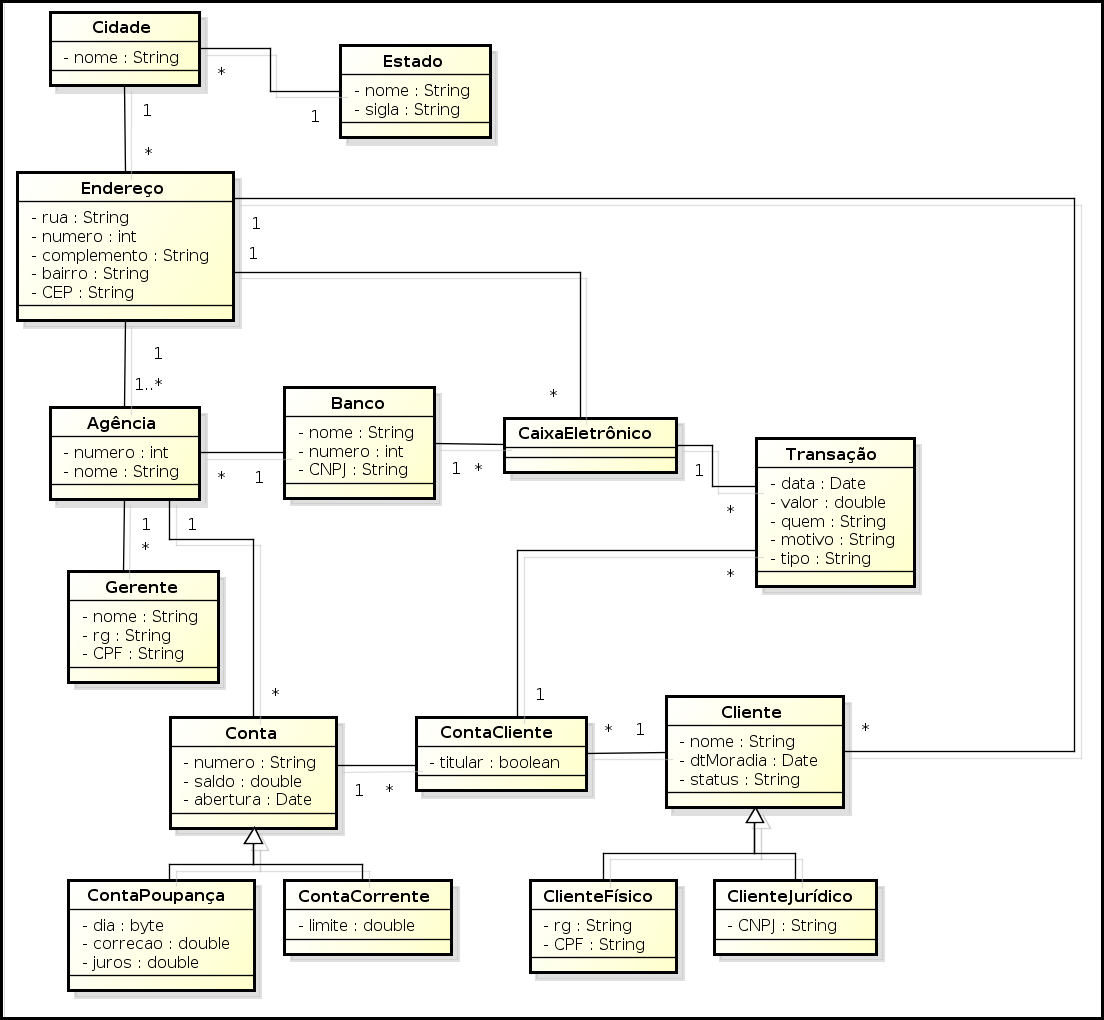
\includegraphics[width=14cm]{fig/ControleBancario}
\caption{Diagrama de classes UML}
\label{figUML}
\end{figure}

\vspace{0.5cm}

\begin{cBox}
{\bf  ControleBancario.} Essa aplicação  controla bancos,  cada um  com diversas
agências nas quais os clientes  podem realizar transações em contas correntes ou
poupanças. Um  cliente é qualquer pessoa  física ou jurídica que  abre uma conta
corrente  ou poupança  em uma  ou mais  agências de  um banco  operado  por essa
aplicação. Assim,  as  contas   estão  vinculadas  às  diferentes  agências  em
diferentes  endereços,  de  várias  cidades  em vários  estados.   Uma  conta  é
associada sempre a um cliente titular  e a zero ou mais outros clientes (segundo
titular, terceiro titular, etc). 

As transações  realizadas pelo cliente  podem ser de  retirada de valor  de suas
contas, de depósito e de transferência de valores entre contas de um mesmo banco.
\end{cBox}

Levando  em consideração o  padrão MVC~\cite{KP88},  as entidades,  presentes na
Figura~\ref{figUML}, fazem parte do modelo (o  M do MVC) da aplicação.  Assim, é
necessário  criar  uma classe  de  Domínio\footnote{Em  Grails,  os modelos  são
  denominados  de classes  de domínio.}   para cada  entidade da  aplicação {\bf
  ControleBancario}\index{Modelo-Visão-Controlador (MVC)!Modelo}.  

\subsection{Classe de Domínio: Estado}\label{secEstado}

\vspace{0.5cm}

A primeira  classe de  domínio a ser  implementada é  a classe {\bf  Estado} que
representa os estados brasileiros.

\begin{itemize}

\item Para criá-la  no IDE IntelliJ, selecione {\bf  New} $\Longrightarrow$ {\bf
  Grails Domain Class} (Figura~\ref{novoEstadoFig}). 

\vspace{0.5cm}

\item Digite  {\bf br.ufscar.dc.dsw.Estado} como o  nome da classe  de domínio e
  clique  em  {\bf  Finish}.  O  IDE  IntelliJ  executa  o comando  {\bf  grails
    create-domain-class}. A  classe de domínio  {\bf Estado.groovy} é  criada no
  diretório {\bf grails-app/domain}. \index{Comandos!grails create-domain-class} 
 
\vspace{0.5cm}

\item  Abra a  classe {\bf  Estado} e  insira os  atributos ({\bf  nome}  e {\bf
  sigla}) dessa classe conforme apresentado no Código~\ref{codEstado}. 

\end{itemize}

\begin{figure}[htbp]
\centering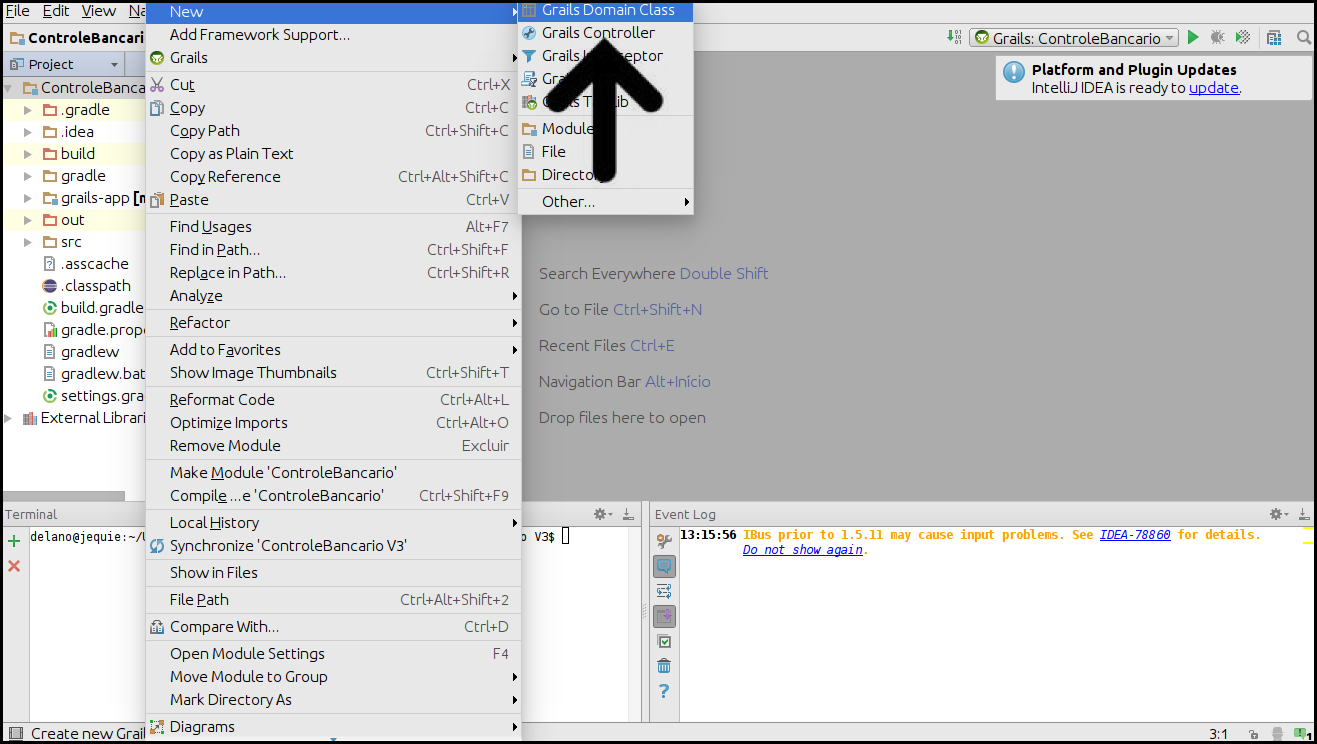
\includegraphics[width=12cm]{criaDomainClass}
\caption{Criação da Classe de Domínio Estado.}
\label{novoEstadoFig}
\end{figure}

\hspace{1cm}\\
\noindent {\bf Observações:}

\begin{itemize}

\item O  atributo {\bf  id} é  gerado automaticamente pelo  Grails. Logo,  não é
  necessário incluí-lo na implementação da classe {\bf Estado}; 

\vspace{0.2cm}

\item A classe de domínio {\bf Estado} possui os seguintes atributos:

\vspace{0.2cm}

\begin{itemize}

\item[$\diamond$] {\bf nome} -- que armazena o nome do estado;

\vspace{0.2cm}

\item[$\diamond$] {\bf  sigla} -- que armazena  a sigla do  estado (por exemplo:
  {\bf SP} para o estado de São Paulo); 

\end{itemize}

\vspace{0.5cm}

\item O método {\bf toString()} retorna  uma representação (por exemplo, o que é
  apresentada nas visões – páginas HTML) das instâncias das classes.  No caso da
  implementação da  classe de  domínio {\bf Estado},  o método  {\bf toString()}
  retorna a sigla do estado.
 
\end{itemize}

\newpage

\begin{lstlisting}[caption=Classe  de  domínio   {\bf  Estado},  frame  =  trBL,
    float=htbp, label=codEstado] 
package br.ufscar.dc.dsw

class Estado {
    static constraints = {
        nome (nullable: false, size: 1..20)
        sigla (nullable: false, size: 2..2)
    }
    
    String nome
    String sigla
    
    String toString() {
        return sigla
    }
}
\end{lstlisting}

\subsubsection{Validação de Dados}\index{Validação de Dados}\label{validacao}

\vspace{0.2cm}

\noindent  O  bloco {\bf  static  constraints}  permite  que os  desenvolvedores
coloquem regras  de validação nas classes  de domínio.  Por  exemplo, é possível
impor restrições  sobre o tamanho  máximo de um  atributo String (por  padrão, o
tamanho é 255 caracteres).  Além disso,  é possível garantir que campos de texto
(Strings) correspondem  a um determinado padrão  (como um endereço  de e-mail ou
URL). E por fim, é possível até mesmo tornar campos opcionais ou obrigatórios.

\vspace{0.2cm}

Além  dessas validações,  o bloco  {\bf static  constraints}  também possibilita
definir a  ordem em que  os atributos de  um modelo são apresentados  nas visões
associadas.   O Código  ~\ref{codEstado} descreve  o  uso do  bloco {\bf  static
  constraints}  para validar os  atributos da  classe {\bf  Estado} e  definir a
ordem   em    que   os   atributos    dessa   classe   são    apresentados.    A
Tabela~\ref{restricoesTbl}   apresenta  algumas   restrições  com   exemplos  de
utilização e respectivas descrições.

\vspace{0.2cm}

\begin{table}[htbp]
\centering
\begin{footnotesize}
\begin{tabular}{p{2.0cm} | p{4.5cm} | p{6.5cm}}
\toprule     
\rowcolor{Gray}     
\textbf{Nome}     &     \textbf{Exemplo}     & \textbf{Descrição}\\  
\midrule 
blank &  nome(blank:false) & Coloque {\bf false}  se o valor da  String não pode
estar em branco.\\
\midrule
email &  e-mail(email:true) & Coloque {\bf  true} se a String  necessitar ser um
endereço de e-mail válido.\\
\midrule 
inList & sexo(inList:["F", "M"]) & O valor deve estar contido
na  lista.  \\  
\midrule  
length &  nome(length:5..15) & Usa  uma faixa para  restringir o tamanho  de uma
String ou array.\\
\midrule
min & quantidade(min:0) & Define o valor mínimo. \\
\midrule 
matches  & nome(matches:/[a-zA-Z]/) &  Verifica se  corresponde a  uma expressão
regular fornecida.  \\
\midrule   
max & quantidade(max:100) & Define o valor máximo. \\
\midrule
nullable &  preco(nullable:false) & Coloque {\bf  false} se o  valor do atributo
não poder ser nulo. \\
\midrule  
range  &  quantidade(range:5..15)  &   Valor  deve  estar  dentro  do  intervalo
especificado.  \\
\midrule  
size  & list(size:5..15)  &  Usa uma  faixa  para restringir  o  tamanho de  uma
coleção.\\
\midrule  
unique & nome(unique:true)  & Defina como {\bf true} se o  valor do atributo não
pode repetir. \\
\midrule
url & homepage(url:true)  & Defina como {\bf true} se o valor da String precisar
ser um endereço URL válido.  \\
\bottomrule
\end{tabular}
\end{footnotesize}
\caption{Regras de restrições.}
\label{restricoesTbl}
\end{table}

\newpage

\subsection{Classe de Domínio: Cidade}\label{secCidade}

\vspace{0.5cm}

A próxima classe de domínio a ser  criada é a classe {\bf Cidade} que representa
cidades  brasileiras.  Crie, usando  os mesmos  passos da  criação da  classe de
domínio {\bf  Estado} (Seção~\ref{secEstado}), a  classe {\bf Cidade}  do pacote
{\bf  br.ufscar.dc.dsw}. Abra  a  classe  {\bf Cidade},  insira  os atributos  e
acrescente as suas validações, conforme apresentado no Código~\ref{codCidade}.  

\begin{lstlisting}[caption=Classe  de  domínio   {\bf  Cidade},  frame  =  trBL,
    float=htbp, label=codCidade] 
package br.ufscar.dc.dsw

class Cidade {

    static constraints = {
        nome (blank: false, size: 1..40)
        estado (nullable: false)
    }

    String nome
    Estado estado
    
    String toString() {
        StringBuilder sb = new StringBuilder();
        if (nome != null) {
            sb.append(nome)
            sb.append(" - ")
            sb.append(estado.sigla)
        }
        return sb.toString();
    }
}
\end{lstlisting}

\hspace{1cm}\\
\noindent {\bf Observações:}
\hspace{1cm}\\

\begin{itemize}

\item A classe de domínio {\bf Cidade} possui os seguintes atributos:

\vspace{0.2cm}

\begin{itemize}

\item[$\diamond$] {\bf nome} -- que armazena o nome da cidade;

\vspace{0.2cm}

\item[$\diamond$] {\bf estado} -- que armazena uma referência a uma instância da
  classe {\bf Estado}.   Esse atributo é um mapeamento  unidirecional entre {\bf
    Cidade} e {\bf  Estado}.  Pelos requisitos da aplicação,  não há necessidade
  de implementar um mapeamento bidirecional entre essas duas classes de domínio.

\end{itemize}

\end{itemize}

\vspace{0.5cm}

\begin{cBox}
Uma  importante característica  do Grails  é que  programadores não  precisam se
preocupar em criar  os métodos {\it getters} e {\it  setters}.  Eles são gerados
pelo Groovy.  Grails, por meio  do mecanismo GORM ({\it Grails Object-Relational
  Mapping})\index{GORM}, realiza um mapeamento automático entre modelos (classes
de domínio) e tabelas em um SGBD.

Dessa forma, o Groovy gera outros métodos estáticos responsáveis pelas operações
{\it CRUD} ({\it Create}, {\it Read}, {\it Update} e {\it Delete}): 

\begin{itemize}

\item {\bf Cidade.save()} armazena os dados na tabela Cidade (do SGBD).

\item {\bf Cidade.delete()} apaga os dados da tabela Cidade.

\item {\bf Cidade.list()} retorna uma lista de cidades.

\item {\bf Cidade.get()} retorna uma única instância da classe Cidade.

\end{itemize}

Todos esses  e outros métodos  estão disponíveis para os  desenvolvedores.  Note
que  {\bf  Cidade}  não  estende  nenhuma  classe  pai  nem  implementa  nenhuma
interface.   Graças  aos  recursos  de  metaprogramação  Groovy,  esses  métodos
simplesmente  aparecem  quando  necessários.   Apenas as  classes  presentes  no
diretório {\bf  grails-app/domain} (ou seja,  classes de domínio)  possuem esses
métodos relacionados à persistência de dados: {\bf save()}, {\bf delete()}, {\bf
  list()} e {\bf get()}.
\end{cBox}

\newpage

\subsection{Classe de Domínio: Endereco}\label{secEndereco}

\vspace{0.5cm}

Crie,  usando os  mesmos passos  da criação  da classe  de domínio  {\bf Estado}
(Seção~\ref{secEstado}),    a   classe   {\bf    Endereco}   do    pacote   {\bf
  br.ufscar.dc.dsw}.   Abra  a classe  {\bf  Endereco},  insira  os atributos  e
acrescente     as      suas     validações,     conforme      apresentado     no
Código~\ref{codEndereco}. 

\begin{lstlisting}[caption=Classe  de  domínio  {\bf  Endereco}, frame  =  trBL,
    float=htbp, label=codEndereco]
package br.ufscar.dc.dsw

class Endereco {

    static constraints = {
        CEP (blank: false, cep: true, size: 9..9)
        logradouro (blank: false, size: 1..40)
        numero (min: 0)
        complemento (nullable: true, size: 1..40)
        bairro (blank: false, size: 1..40)
        cidade (nullable: false)
    }
    
    String logradouro
    
    int numero
    
    String complemento
    
    String bairro
    
    String CEP
    
    Cidade cidade
    
    String toString() {
        return logradouro + ", " + numero + 
               (complemento == null ? "" : " " + complemento) + ". " + 
               bairro + " " + CEP + " " + cidade 
    }
}
\end{lstlisting}

\hspace{1cm}\\
\noindent {\bf Observações:}
\hspace{1cm}\\

\begin{itemize}

\item A classe de domínio {\bf Endereco} possui os seguintes atributos:

\vspace{0.5cm}

\begin{itemize}

\item[$\diamond$] {\bf logradouro} -- que armazena o nome do logradouro;

\vspace{0.5cm}

\item[$\diamond$] {\bf numero} -- que armazena o número do endereço;

\vspace{0.5cm}

\item[$\diamond$] {\bf complemento} -- que armazena o complemento de endereço;

\vspace{0.5cm}

\item[$\diamond$] {\bf bairro} -- que armazena o bairro do endereço;

\vspace{0.5cm}

\item[$\diamond$] {\bf CEP} -- que armazena o CEP de endereço. A validação desse
  atributo utiliza a  restrição {\bf cep: true} definida  pelo {\it plugin} {\bf
    br-validation} instalado na Seção~\ref{secPlugins}; e

\vspace{0.5cm}

\item[$\diamond$] {\bf cidade} -- que armazena uma referência a uma instância da
  classe  {\bf Cidade}  (Seção~\ref{secCidade}). Esse  atributo é  um mapeamento
  unidirecional  entre  {\bf Endereco}  e  {\bf  Cidade}.   Pelos requisitos  da
  aplicação, não há necessidade  de implementar um mapeamento bidirecional entre
  essas duas classes de domínio.  

\end{itemize}

\vspace{0.5cm}

\item O  método {\bf  toString()} retorna uma  representação das  instâncias das
  classes.   No caso da  implementação da  classe de  domínio {\bf  Endereco}, o
  método  {\bf  toString()} retorna  uma  descrição  textual  do endereço  (rua,
  número, complemento, bairro, CEP e cidade).

\end{itemize}

\newpage

\subsection{Classe de Domínio: Banco}\label{secBanco}

\vspace{0.5cm}

A próxima classe de  domínio a ser criada é a classe  {\bf Banco} que representa
instituições bancárias.  Crie,  usando os mesmos passos da  criação da classe de
domínio  {\bf Estado} (Seção~\ref{secEstado}),  a classe  {\bf Banco}  do pacote
{\bf  br.ufscar.dc.dsw}.  Abra  a  classe  {\bf Banco},  insira  os atributos  e
acrescente as suas validações, conforme apresentado no Código~\ref{codBanco}. 

\begin{lstlisting}[caption=Classe  de   domínio  {\bf  Banco},   frame  =  trBL,
    float=htbp, label=codBanco] 
package br.ufscar.dc.dsw

class Banco {

    static hasMany = [agencias: Agencia, caixas: CaixaEletronico]

    static constraints = {
        numero (unique: true, min: 0)
        nome (blank: false, size: 1..20)
        CNPJ (blank: false, unique:true, cnpj: true, size: 18..18)
    }

    int numero
    String nome
    String CNPJ

    String toString() {
        return nome
    }
}
\end{lstlisting}

\hspace{1cm}\\
\noindent {\bf Observações:}
\hspace{1cm}\\

\begin{itemize}

\item A classe de domínio {\bf Banco} possui os seguintes atributos:

\vspace{0.5cm}

\begin{itemize}

\item[$\diamond$] {\bf numero}  -- que armazena o número  (único) da instituição
  bancária; 

\vspace{0.5cm}

\item[$\diamond$] {\bf nome} -- que armazena o nome da instituição bancária; e

\vspace{0.5cm}

\item[$\diamond$] {\bf CNPJ} -- que  armazena o CNPJ da instituição bancária.  A
  validação desse  atributo utiliza a  restrição {\bf cnpj: true}  definida pelo
  {\it plugin} {\bf br-validation} instalado na Seção~\ref{secPlugins}.

\end{itemize}

\vspace{0.5cm}

\item O comando {\bf static hasMany  = [agencias: Agencia]} na classe de domínio
  {\bf  Banco} e  o atributo  {\bf  banco} na  classe de  domínio {\bf  Agencia}
  (Seção~\ref{secAgencia}),  foram utilizados  em conjunto  para  implementar um
  mapeamento {\em um-para-muitos} entre essas classes.
 
\vspace{0.5cm}

\item O  comando {\bf static hasMany  = [caixas: CaixaEletronico]}  na classe de
  domínio  {\bf Banco}  e  o atributo  {\bf  banco} na  classe  de domínio  {\bf
    CaixaEletronico}   (Seção~\ref{secCaixaEletronico}),  foram   utilizados  em
  conjunto  para  implementar um  mapeamento  {\em  um-para-muitos} entre  essas
  classes.

\vspace{0.5cm}

\item O  método {\bf  toString()} retorna uma  representação das  instâncias das
  classes.  No caso da implementação da  classe de domínio {\bf Banco}, o método
  {\bf toString()} retorna apenas o nome do banco.

\end{itemize}

\newpage

\subsection{Classe de Domínio: Agencia}\label{secAgencia}

\vspace{0.5cm}

A  classe   de  domínio  {\bf  Agencia}  representa   agências  de  instituições
bancárias. Crie a classe {\bf Agencia} do pacote {\bf br.ufscar.dc.dsw}.  Abra a
classe  {\bf Agencia},  insira os  atributos  e acrescente  as suas  validações,
conforme apresentado no Código~\ref{codCidade}. 

\begin{lstlisting}[caption=Classe  de  domínio  {\bf  Agencia},  frame  =  trBL,
    float=htbp, label=codAgencia] 
package br.ufscar.dc.dsw

class Agencia {

    static hasMany = [gerentes: Gerente]

    static constraints = {
        banco (nullable: false)
        numero (blank: false, min: 0)
        nome (blank: false, size: 1..20)
        endereco (nullable: false)
    }

    int numero
    String nome
    Endereco endereco
    Banco banco

    String toString() {
        StringBuilder sb = new StringBuilder();
        sb.append(numero)
        sb.append(" - ")
        sb.append(banco)
        return sb.toString();
    }
}
\end{lstlisting}

\vspace{0.3cm}
\noindent {\bf Observações:}
\hspace{1cm}\\

\begin{itemize}

\item A classe de domínio {\bf Agencia} possui os seguintes atributos:

\vspace{0.5cm}

\begin{itemize}

\item[$\diamond$] {\bf numero} -- que armazena o número da agência bancária; 

\vspace{0.5cm}

\item[$\diamond$] {\bf nome} -- que armazena o nome da agência bancária; 

\vspace{0.5cm}

\hyphenation{Endereco}
\hyphenation{Agencia}

\item[$\diamond$] {\bf endereco} -- que  armazena uma referência a uma instância
  da classe de domínio  {\bf Endereco} (Seção~\ref{secEndereco}).  Esse atributo
  é um  mapeamento unidirecional  entre {\bf Agencia}  e {\bf  Endereco}.  Pelos
  requisitos  da aplicação,  não  há necessidade  de  implementar um  mapeamento
  bidirecional entre essas duas classes de domínio; e

\vspace{0.5cm}

\item[$\diamond$] {\bf banco} -- que  armazena uma referência a uma instância da
  classe   de  domínio  {\bf   Banco}  (Seção~\ref{secBanco}).    Esse  atributo
  representa a cardinalidade {\em ``um''} do relacionamento {\em um-para-muitos}
  entre as classes de domínio {\bf Banco} e {\bf Agencia}.

\end{itemize}

\vspace{0.5cm}

\item O comando {\bf static hasMany  = [gerentes: Gerente]} na classe de domínio
  {\bf Agencia}  e o atributo {\bf  agencia} na classe de  domínio {\bf Gerente}
  (Seção~\ref{secGerente}),  foram  utilizados em  conjunto  para implementar  o
  mapeamento  {\em  um-para-muitos}  entre  as  classes  {\bf  Agencia}  e  {\bf
    Gerente}.

\vspace{0.5cm}

\item O  método {\bf  toString()} retorna uma  representação das  instâncias das
  classes.   No caso  da implementação  da classe  de domínio  {\bf  Agencia}, o
  método {\bf toString()} retorna o número  da agência concatenado com o nome do
  banco.

\end{itemize}

\newpage

\subsection{Classe de Domínio: Gerente}\label{secGerente}

\vspace{0.5cm}

A  classe  de   domínio  {\bf  Gerente}  representa  gerentes   de  agências  de
instituições   bancárias.  Crie   a  classe   {\bf  Gerente}   do   pacote  {\bf
  br.ufscar.dc.dsw}.   Abra  a  classe  {\bf  Gerente}, insira  os  atributos  e
acrescente as suas validações, conforme apresentado no Código~\ref{codGerente}.  

\begin{lstlisting}[caption=Classe  de  domínio  {\bf  Gerente},  frame  =  trBL,
    float=htbp, label=codGerente] 
package br.ufscar.dc.dsw

class Gerente {

    static constraints = {
        nome (blank: false, size: 1..30)
        rg (blank: false, size: 1..12)
        CPF (blank: false, unique: true, cpf: true, size: 14..14)
        agencia (nullable: false)
    }

    String nome
    String rg
    String CPF
    Agencia agencia
    
    String toString() {
        return nome + " " + CPF
    }
}
\end{lstlisting}

\hspace{1cm}\\
\noindent {\bf Observações:}
\hspace{1cm}\\

\begin{itemize}

\item A classe de domínio {\bf Gerente} possui os seguintes atributos:

\vspace{0.5cm}

\begin{itemize}

\item[$\diamond$] {\bf nome} -- que armazena o nome do gerente; 

\vspace{0.5cm}

\item[$\diamond$] {\bf rg} -- que armazena o RG do gerente; 

\vspace{0.5cm}

\item[$\diamond$] {\bf CPF} -- que  armazena o CPF do gerente.  A
  validação desse  atributo utiliza a  restrição {\bf cpf: true}  definida pelo
  {\it plugin} {\bf br-validation} instalado na Seção~\ref{secPlugins}; e

\vspace{0.5cm}

\hyphenation{Agencia}

\item[$\diamond$] {\bf agencia}  -- que armazena uma referência  a uma instância
  da classe  de domínio  {\bf Agencia} (Seção~\ref{secAgencia}).   Esse atributo
  representa a cardinalidade {\em ``um''} do relacionamento {\em um-para-muitos}
  entre as classes de domínio {\bf Agencia} e {\bf Gerente}.

\end{itemize}

\vspace{0.5cm}

\item O  método {\bf  toString()} retorna uma  representação das  instâncias das
  classes.   No caso  da implementação  da classe  de domínio  {\bf  Gerente}, o
  método  {\bf  toString()}  retorna  o  nome do  gerente  concatenado  com  seu
  respectivo CPF.

\end{itemize}

\newpage

\subsection{Classe de Domínio: CaixaEletronico}\label{secCaixaEletronico}

\vspace{0.5cm}

\hyphenation{CaixaEletronico}

A  classe  de  domínio  {\bf  CaixaEletronico}  representa  caixas  eletrônicos,
pertencentes    às   instituições    bancárias,   onde    transações   bancárias
(Seção~\ref{secTransacao})   podem   ser  realizadas.    Crie   a  classe   {\bf
  CaixaEletronico}  do  pacote  {\bf  br.ufscar.dc.dsw}.   Abra  a  classe  {\bf
  CaixaEletronico},  insira  os  atributos  e  acrescente  as  suas  validações,
conforme apresentado no Código~\ref{codCaixaEletronico}. 

\begin{lstlisting}[caption=Classe  de  domínio  {\bf CaixaEletronico},  frame  =
    trBL, float=htbp, label=codCaixaEletronico] 
package br.ufscar.dc.dsw

class CaixaEletronico {

    static hasMany = [transacoes: Transacao]
    
    static constraints = {
        banco (nullable: false)
        endereco (nullable: false)
    }
    
    Endereco endereco
    Banco banco
    
    String toString() {
        return banco.toString() + " - " + endereco.toString();
    }
}
\end{lstlisting}

\hspace{1cm}\\
\noindent {\bf Observações:}
\hspace{1cm}\\

\begin{itemize}

\item A classe de domínio {\bf CaixaEletronico} possui os seguintes atributos: 

\vspace{0.5cm}

\begin{itemize}

\item[$\diamond$] {\bf banco} -- que  armazena uma referência a uma instância da
  classe de domínio {\bf  Banco} (Seção~\ref{secBanco}).  Ou seja, esse atributo
  representa a cardinalidade {\em ``um''} do relacionamento {\em um-para-muitos}
  entre as classes de domínio {\bf Banco} e {\bf CaixaEletronico};

\vspace{0.5cm}

\hyphenation{CaixaEletronico}
\item[$\diamond$] {\bf endereco} -- que  armazena uma referência a uma instância
  da classe de domínio  {\bf Endereco} (Seção~\ref{secEndereco}).  Esse atributo
  é um  mapeamento unidirecional entre  {\bf CaixaEletronico} e  {\bf Endereco}.
  Pelos requisitos da aplicação, não há necessidade de implementar um mapeamento
  bidirecional entre essas duas classes de domínio.

\end{itemize}

\vspace{0.5cm}

\item  O comando {\bf  static hasMany  = [transacoes:  Transacao]} na  classe de
  domínio {\bf CaixaEletronico} e o  atributo {\bf caixaEletronico} na classe de
  domínio  {\bf  Transacao}   (Seção~\ref{secTransacao}),  foram  utilizados  em
  conjunto  para  implementar  o  mapeamento {\em  um-para-muitos}  entre  essas
  classes de domínio.

\vspace{0.5cm}

\item O  método {\bf  toString()} retorna uma  representação das  instâncias das
  classes.  No caso da implementação da classe de domínio {\bf CaixaEletronico},
  o método {\bf  toString()} retorna o nome do banco  concatenado com o endereço
  do caixa eletrônico.

\end{itemize}

\newpage

\subsection{Classe de Domínio: Transacao}\label{secTransacao}

\vspace{0.3cm}

A classe de  domínio {\bf Transacao} representa transações  realizadas em contas
bancárias vinculadas a clientes do  banco.  Pelos requisitos da aplicação, todas
as transações bancárias são realizadas em um caixa eletrônico.

\vspace{0.2cm}

Crie a classe  {\bf Transacao} do pacote {\bf  br.ufscar.dc.dsw}.  Abra a classe
{\bf Transacao}, insira  os atributos e acrescente as  suas validações, conforme
apresentado no Código~\ref{codTransacao}.  

\begin{lstlisting}[caption=Classe  de  domínio {\bf  Transacao},  frame =  trBL,
    float=htbp, label=codTransacao] 
package br.ufscar.dc.dsw

class Transacao {
    public static final String CR^É^DITO = "CR^É^DITO"
    public static final String D^É^BITO = "D^É^BITO"
    
    static constraints = {
        contaCliente (nullable: false)
        caixaEletronico (nullable: false)
        valor (nullable: false, min: 0.1d)
        data (nullable: false)
        quem (nullable: false)
        motivo (nullable: false)
        tipo (nullable: false, inList: [CR^É^DITO,D^É^BITO])
    }
        
    Date data
    
    double valor
    
    String quem
    
    String motivo
    
    String tipo
    
    ContaCliente contaCliente
    
    CaixaEletronico caixaEletronico

    String toString() {
        return "[" + tipo + "] - " + motivo + " - R\$ " + valor 
    }
}
\end{lstlisting}

\noindent {\bf Observações:}
\hspace{1cm}\\

\begin{itemize}

\item A classe de domínio {\bf Transacao} possui os seguintes atributos:

\vspace{0.3cm}

\begin{itemize}

\item[$\diamond$] {\bf data} -- que armazena a data em que ocorreu a transação; 

\vspace{0.3cm}

\item[$\diamond$] {\bf valor} -- que armazena o valor da transação; 

\vspace{0.3cm}

\item[$\diamond$] {\bf quem} -- que armazena {\em quem} realizou a transação; 

\vspace{0.3cm}

\item[$\diamond$] {\bf motivo} -- que  armazena {\em o motivo} (saque, depósito,
  transferência) da transação;

\vspace{0.3cm}

\item[$\diamond$] {\bf tipo} -- que  armazena o tipo de transação: {\bf Crédito}
  ou {\bf Débito};

\vspace{0.3cm}

\item[$\diamond$]  {\bf  contaCliente} --  que  armazena  uma  referência a  uma
  instância      da      classe      de     domínio      {\bf      ContaCliente}
  (Seção~\ref{secContaCliente}).  Esse atributo  representa a cardinalidade {\em
    ``um''} do  relacionamento {\em  um-para-muitos} entre {\bf  ContaCliente} e
  {\bf Transacao}. 

\vspace{0.3cm}

\item[$\diamond$]  {\bf caixaEletronico} --  que armazena  uma referência  a uma
  instância     da      classe     de     domínio      {\bf     CaixaEletronico}
  (Seção~\ref{secCaixaEletronico}).   Ou   seja,  esse  atributo   representa  a
  cardinalidade {\em  ``um''} do relacionamento {\em  um-para-muitos} entre {\bf
    CaixaEletronico} e {\bf Transacao}. 

\end{itemize}

\end{itemize}

\newpage

\subsection{Classe de Domínio: ContaCliente}\label{secContaCliente}

\vspace{0.5cm}

A  classe  de  domínio  {\bf  ContaCliente} materializa  o  relacionamento  {\em
  muitos-para-muitos} entre as classes de domínio {\bf Conta} e {\bf Cliente}. O
relacionamento  {\em muitos-para-muitos}  entre {\bf  Conta} e  {\bf  Cliente} é
obtido ao implementar dois relacionamentos {\em um-para-muitos}: (i) {\bf Conta}
x {\bf ContaCliente} e (ii) {\bf Cliente} x {\bf ContaCliente}.

\vspace{0.2cm}

Crie  a classe  {\bf ContaCliente}  do  pacote {\bf  br.ufscar.dc.dsw}.  Abra  a
classe {\bf ContaCliente}, insira os  atributos e acrescente as suas validações,
conforme apresentado no Código~\ref{codContaCliente}.  

\begin{lstlisting}[caption=Classe de  domínio {\bf ContaCliente},  frame = trBL,
    float=htbp, label=codContaCliente] 
package br.ufscar.dc.dsw

class ContaCliente {

    static hasMany = [transacoes: Transacao]
    
    static constraints = {
        cliente (nullable: false)
        conta (nullable: false, unique: 'cliente')
        titular (nullable: false)
    }
    
    boolean titular
    Conta conta
    Cliente cliente
    
    String toString() {
        return cliente.toString() + " X " + conta
    }
}
\end{lstlisting}

\hspace{1cm}\\
\noindent {\bf Observações:}
\hspace{1cm}\\

\begin{itemize}

\item A classe de domínio {\bf ContaCliente} possui os seguintes atributos:

\vspace{0.5cm}

\begin{itemize}

\item[$\diamond$]  {\bf titular}  -- que  determina se  o cliente  é  titular da
  conta; 

\vspace{0.5cm}

\item[$\diamond$] {\bf conta} -- que  armazena uma referência a uma instância da
  classe   de  domínio  {\bf   Conta}  (Seção~\ref{secConta}).    Esse  atributo
  representa a cardinalidade {\em ``um''} do relacionamento {\em um-para-muitos}
  entre as classes de domínio {\bf Conta} e {\bf ContaCliente}; e

\vspace{0.5cm}

\item[$\diamond$] {\bf cliente}  -- que armazena uma referência  a uma instância
  da classe  de domínio  {\bf Cliente} (Seção~\ref{secCliente}).   Esse atributo
  representa a cardinalidade {\em ``um''} do relacionamento {\em um-para-muitos}
  entre as classes de domínio {\bf Cliente} e {\bf ContaCliente}.

\end{itemize}

\vspace{0.5cm}

\hyphenation{ContaCliente}

\item  O comando {\bf  static hasMany  = [transacoes:  Transacao]} na  classe de
  domínio  {\bf ContaCliente}  e  o  atributo {\bf  contaCliente}  na classe  de
  domínio  {\bf  Transacao}   (Seção~\ref{secTransacao}),  foram  utilizados  em
  conjunto  para  implementar um  mapeamento  {\em  um-para-muitos} entre  essas
  classes.

\vspace{0.5cm}

\item O  método {\bf  toString()} retorna uma  representação das  instâncias das
  classes.  No caso da implementação  da classe de domínio {\bf ContaCliente}, o
  método {\bf toString()}  retorna a concatenação das representações  da conta e
  do cliente associados à essa instância da classe {\bf ContaCliente}.

\end{itemize}

\newpage

\subsection{Classe de Domínio: Conta}\label{secConta}

\vspace{0.5cm}

A classe de domínio {\bf Conta} representa contas bancárias. Pelos requisitos da
aplicação, a classe {\bf Conta} é  abstrata e portanto instâncias de {\bf Conta}
não  podem  ser  criadas  -  apenas  de  suas  subclasses:  {\bf  ContaCorrente}
(Seção~\ref{secContaCorrente})           e          {\bf          ContaPoupanca}
(Seção~\ref{secContaPoupanca}). 

\vspace{0.2cm}

Crie a classe {\bf Conta} do  pacote {\bf br.ufscar.dc.dsw}.  Abra a classe {\bf
  Conta},  insira  os  atributos  e  acrescente  as  suas  validações,  conforme
apresentado no Código~\ref{codConta}.  

\begin{lstlisting}[caption=Classe  de   domínio  {\bf  Conta},   frame  =  trBL,
    float=htbp, label=codConta] 
package br.ufscar.dc.dsw

abstract class Conta {

    static hasMany = [contasCliente: ContaCliente]
    
    static constraints = {
        numero (blank: false)
        agencia (nullable: false)
        saldo (nullable: false, min: 0.0d)
        abertura (nullable: false)
    }
	
    static mapping = {
        tablePerHierarchy false
    }
        
    Agencia agencia
    
    String numero
	
    double saldo
	
    Date abertura
	
}
\end{lstlisting}

\hspace{1cm}\\
\noindent {\bf Observações:}
\hspace{1cm}\\

\begin{itemize}

\item A classe de domínio abstrata {\bf Conta} possui os seguintes atributos:

\vspace{0.5cm}

\begin{itemize}

\item[$\diamond$] {\bf agencia}  -- que armazena uma referência  a uma instância
  da  classe  {\bf  Agencia}   (Seção~\ref{secAgencia}).   Esse  atributo  é  um
  mapeamento unidirecional entre {\bf  Conta} e {\bf Agencia}.  Pelos requisitos
  da  aplicação, não há  necessidade de  implementar um  mapeamento bidirecional
  entre essas duas classes de domínio;

\vspace{0.5cm}

\item[$\diamond$] {\bf numero} -- que armazena o número da conta bancária; 

\vspace{0.5cm}

\item[$\diamond$] {\bf saldo} -- que armazena o saldo da conta bancária; e

\vspace{0.5cm}

\item[$\diamond$] {\bf  abertura} --  que armazena a  data de abertura  da conta
  bancária; 

\end{itemize}

\vspace{0.5cm}

\item O comando  {\bf static hasMany = [contasCliente:  ContaCliente]} na classe
  de domínio  {\bf Conta}  e o atributo  {\bf conta}  na classe de  domínio {\bf
    ContaCliente}  (Seção~\ref{secContaCliente}), foram  utilizados  em conjunto
  para implementar um mapeamento {\em um-para-muitos} entre essas classes.

\end{itemize}

\newpage

\subsection{Classe de Domínio: ContaCorrente}\label{secContaCorrente}

\vspace{0.5cm}

A classe  de domínio {\bf  ContaCorrente}, subclasse de {\bf  Conta}, representa
contas correntes.  O atributo {\bf limite} representa o limite (cheque especial)
que a  instituição bancária  disponibiliza ao cliente  caso necessário.   Crie a
classe {\bf ContaCorrente} do pacote {\bf br.ufscar.dc.dsw}.  Abra a classe {\bf
  ContaCorrente}, insira os atributos  e acrescente as suas validações, conforme
apresentado no Código~\ref{codContaCorrente}. 

\begin{lstlisting}[caption=Classe de domínio  {\bf ContaCorrente}, frame = trBL,
    float=htbp, label=codContaCorrente] 
package br.ufscar.dc.dsw

class ContaCorrente extends Conta{

    static constraints = {
        numero (blank: false)
        agencia (nullable: false)
        saldo (nullable: false, min: 0.0d)
        limite (nullable: false, min: 0.0d)
        abertura (nullable: false)
    }
    
    double limite
    
    String toString() {
        return "(Conta Corrente) " + numero
    }
}
\end{lstlisting}

\subsection{Classe de Domínio: ContaPoupanca}\label{secContaPoupanca}

\vspace{0.5cm}

A classe  de domínio {\bf  ContaPoupanca}, subclasse de {\bf  Conta}, representa
contas de  poupança, que  também são chamadas  de {\em cadernetas  de poupança}.
Crie  a classe  {\bf ContaPoupanca}  do pacote  {\bf br.ufscar.dc.dsw}.   Abra a
classe {\bf ContaPoupanca}, insira os atributos e acrescente as suas validações,
conforme apresentado no Código~\ref{codContaPoupanca}. 

\begin{lstlisting}[caption=Classe de domínio  {\bf ContaPoupanca}, frame = trBL,
    float=htbp, label=codContaPoupanca] 
package br.ufscar.dc.dsw

class ContaPoupanca extends Conta{

    static constraints = {
        numero (blank: false)
        agencia (nullable: false)
        saldo (nullable: false, min: 0.0d)
        juros (min: 0.0d)
        correcao (min: 0.0d)
        dia (blank: false, range: 1..28)
        abertura (nullable: false)
    }
    
    
    byte dia    
    double correcao
    double juros
    
    String toString() {
        return "(Poupan^ç^a) " + numero
    }
}
\end{lstlisting}

A classe de domínio {\bf  ContaPoupanca} possui os seguintes atributos: (i) {\bf
  dia} que  armazena o dia  de aniversário da  caderneta de poupança;  (ii) {\bf
  correcao} que armazena o valor de  correção mensal da caderneta de poupança; e
(iii) {\bf juros} que armazena o valor dos juros de reajuste mensal da caderneta
de poupança.

\newpage

\subsubsection{{\it GORM:} Relacionamento de herança}
\index{GORM!Relacionamento de herança}\label{secGORM}

\vspace{0.5cm}

O  mecanismo  GORM  ({\it   Grails  Object-Relational  Mapping})  dá  suporte  à
implementação de herança de classes de entidades abstratas e concretas. Ou seja,
possibilita o mapeamento do modelo de  objetos para o modelo de dados relacional
e vice-versa

\vspace{0.2cm}

Por  {\it default}, o  mecanismo GORM  utiliza a  estratégia de  mapeamento {\it
  table-per-hierarchy} (ver  Figura~\ref{gormFig}(a)) que consiste  em uma única
tabela para toda a hierarquia.  Essa  tabela armazena os atributos da classe pai
({\bf  Conta})  bem  como  os  atributos  específicos  de  cada  subclasse  {\bf
  ContaCorrente} e {\bf ContaPoupanca}  e contem ainda uma coluna discriminadora
denominada {\bf class}.  Essa coluna  mantém valores de marcação que informam ao
framework {\it  hibernate} qual subclasse  instanciar durante a  recuperação dos
dados do SGBD.

\begin{figure}[h]
\center
\subfigure[{\it table-per-hierarchy}]{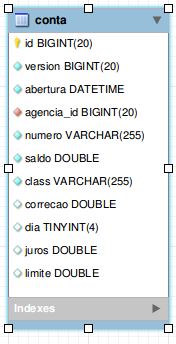
\includegraphics[height=7cm]{tablePerHierarchy}}
\qquad
\subfigure[{\it table-per-class}]{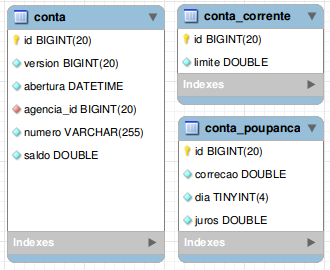
\includegraphics[height=5cm]{tablePerClass}}
\caption{GORM: Mapeamento de Hierarquia}
\label{gormFig}
\end{figure}

Porém, se o {\it default}  da estratégia de mapeamento {\it table-per-hierarchy}
não for  a mais adequada  para sua aplicação,  o desenvolvedor pode  utilizar um
mapeamento    alternativo     --    a    estratégia     {\it    table-per-class}
(Figura~\ref{gormFig}(b)). Nesse  caso, é  criada uma tabela  para a  classe pai
assim  como  para  cada  classe  filha.  Em nosso  exemplo,  a  estratégia  {\it
  table-per-class}  é habilitada  ao incluir  o trecho  apresentado a  seguir na
classe {\bf Conta} (pai da hierarquia).

\begin{cBox}
\begin{verbatim}
static mapping = {
    tablePerHierarchy false
}
\end{verbatim}
\end{cBox}

Pela  Figura~\ref{gormFig}(b), pode-se observar  que foi  criada uma  tabela que
armazena os atributos específicos de cada classe: {\bf Conta}) e suas subclasses
{\bf ContaCorrente} e {\bf ContaPoupanca}.

\newpage

\subsection{Classe de Domínio: Cliente}\label{secCliente}

\vspace{0.5cm}

A  classe  de  domínio  {\bf  Cliente}  representa  clientes  (correntistas)  de
instituições bancárias. Pelos requisitos da  aplicação, a classe {\bf Cliente} é
abstrata e portanto instâncias de {\bf Cliente} não podem ser criadas. Apenas de
suas  subclasses   {\bf  ClienteFisico}   e  {\bf  ClienteJuridico}   podem  ser
instanciadas.

\vspace{0.2cm}

Crie a  classe {\bf Cliente} do  pacote {\bf br.ufscar.dc.dsw}.   Na classe {\bf
  Cliente},  insira  os atributos  e  acrescente  as  suas validações,  conforme
apresentado no Código~\ref{codCliente}. 

\begin{lstlisting}[caption=Classe  de  domínio  {\bf  Cliente},  frame  =  trBL,
    float=htbp, label=codCliente] 
package br.ufscar.dc.dsw

abstract class Cliente {

    static hasMany = [contasCliente: ContaCliente]
    
    public static final String ATIVO = "Ativo"
    public static final String INATIVO = "Inativo"
    
    static constraints = {
        nome (blank: false, size: 1..30)
        endereco (nullable: false)
        dtMoradia (blank: false)
        status (blank: false, inList: [ATIVO, INATIVO])
    }
    
    static mapping = { 
        tablePerHierarchy false
    }
    
    String nome
    String status
    Endereco endereco
    Date dtMoradia
}
\end{lstlisting}

\hspace{1cm}\\
\noindent {\bf Observações:}
\hspace{1cm}\\

\begin{itemize}

\item A classe de domínio abstrata {\bf Cliente} possui os seguintes atributos:

\vspace{0.5cm}

\begin{itemize}

\item[$\diamond$] {\bf nome} -- que armazena o nome do cliente; 

\vspace{0.5cm}

\item[$\diamond$] {\bf status}  -- que armazena o {\it  status} do cliente: {\bf
  Ativo} ou {\bf Inativo};

\vspace{0.5cm}

\item[$\diamond$] {\bf endereco} -- que  armazena uma referência a uma instância
  da  classe  {\bf  Endereco}  (Seção~\ref{secEndereco}).  Esse  atributo  é  um
  mapeamento  unidirecional  entre  {\bf   Cliente}  e  {\bf  Endereco}.   Pelos
  requisitos  da aplicação,  não  há necessidade  de  implementar um  mapeamento
  bidirecional entre essas duas classes de domínio; e

\vspace{0.5cm}

\item[$\diamond$] {\bf dtMoradia} -- que  armazena desde quando o cliente reside
  no endereço armazenado no atributo {\bf endereco}.

\end{itemize}

\vspace{0.5cm}

\item O comando  {\bf static hasMany = [contasCliente:  ContaCliente]} na classe
  {\bf Cliente} e  o atributo {\bf cliente} na  classe {\bf ContaCliente}, foram
  utilizados  em conjunto  para implementar  um mapeamento  {\em um-para-muitos}
  entre essas classes.

\vspace{0.5cm}

\item Análoga  à classe {\bf  Conta}, a classe  de domínio {\bf  Cliente} também
  adota     a     estratégia     {\it     table-per-class}     no     mapeamento
  objeto-relacional. Portanto,  será criada uma  tabela para a classe  pai ({\bf
    Cliente})  assim  como  para  cada  subclasse: {\bf  ClienteFisico}  e  {\bf
    ClienteJuridico}.

\end{itemize}

\newpage

\subsection{Classe de Domínio: ClienteFisico}\label{secClienteFisico}

\vspace{0.5cm}

A classe de domínio {\bf  ClienteFisico}, subclasse de {\bf Cliente}, representa
clientes físicos  de instituições bancárias. Os  atributos {\bf rg}  e {\bf CPF}
armazenam respectivamente a  identidade e o número do  Cadastro de Pessoa Física
desses clientes.  

\vspace{0.2cm}

Crie  a classe  {\bf ClienteFisico}  do pacote  {\bf br.ufscar.dc.dsw}.   Abra a
classe {\bf ClienteFisico}, insira os atributos e acrescente as suas validações,
conforme  apresentado   no  Código~\ref{codClienteFisico}.  Salienta-se   que  a
validação do  atributo {\bf  CPF} utiliza a  restrição {\bf cpf:  true} definida
pelo {\it plugin} {\bf br-validation} instalado na Seção~\ref{secPlugins}. 

\begin{lstlisting}[caption=Classe de domínio  {\bf ClienteFisico}, frame = trBL,
    float=htbp, label=codClienteFisico] 
package br.ufscar.dc.dsw

class ClienteFisico extends Cliente{
    
    static constraints = {
        nome (blank: false, size: 1..30)
        rg (blank: false, size: 1..12)
        CPF (blank: false, unique:true, cpf: true, size: 14..14)
        endereco (nullable: false)
        dtMoradia (blank: false)
        status (blank: false, inList: [ATIVO, INATIVO])
    }
    
    String rg    
    String CPF
    
    String toString() {
        return CPF
    }
}
\end{lstlisting}

\subsection{Classe de Domínio: ClienteJuridico}\label{secClienteJuridico}

\vspace{0.5cm}

A  classe  de  domínio   {\bf  ClienteJurídico},  subclasse  de  {\bf  Cliente},
representa clientes  jurídicos de instituições bancárias. O  atributo {\bf CNPJ}
armazena o número do Cadastro Nacional de Pessoas Jurídicas desses clientes. 

\vspace{0.2cm}

Crie a  classe {\bf ClienteJuridico}  do pacote {\bf br.ufscar.dc.dsw}.   Abra a
classe  {\bf  ClienteJuridico},  insira   os  atributos  e  acrescente  as  suas
validações,    conforme    apresentado    no    Código~\ref{codClienteJuridico}.
Salienta-se  que a validação  do atributo  {\bf CNPJ}  utiliza a  restrição {\bf
  cnpj:  true}  definida pelo  {\it  plugin}  {\bf  br-validation} instalado  na
Seção~\ref{secPlugins}. 

\begin{lstlisting}[caption=Classe  de  domínio  {\bf ClienteJuridico},  frame  =
    trBL, float=htbp, label=codClienteJuridico] 
package br.ufscar.dc.dsw

class ClienteJuridico extends Cliente{
    
    static constraints = {
        nome (blank: false, size: 1..30)
        CNPJ (blank: false, unique:true, cnpj: true, size: 18..18)
        endereco (nullable: false)
        dtMoradia (blank: false)
        status (blank: false, inList: [ATIVO, INATIVO])
    }
    
    String CNPJ
    
    String toString() {
        return CNPJ
    }
}
\end{lstlisting}

\newpage

\section{Scaffolding}\index{Scaffolding}\label{Scaffolding}
\index{Modelo-Visão-Controlador (MVC)!Controlador}
\index{Modelo-Visão-Controlador (MVC)!Visão}

Uma  vez  que  as  classes  de   domínio  estão  criadas,  é  preciso  criar  os
controladores e as  visões relacionados a essas classes  de domínio.  Na geração
de tais artefatos de software será utilizada a abordagem {\it scaffolding} que é
um termo cunhado  pelo framework Rails e adotado pelo Grails  para a geração dos
artefatos (controladores, visões, etc.)  que implementam as operações CRUD. Esse
termo  foi estendido  e atualmente  é possível  criar código  de  autenticação e
autorização,  testes  unitários, dentre  outras  operações.  Em  Grails, o  {\it
  scaffolding}  pode   ser  dinâmico  ou  estático.    Discutiremos  essas  duas
abordagens distintas nas próximas subseções.

\subsection{Scaffolding Dinâmico}\index{Scaffolding!Dinâmico}

\vspace{0.3cm}

No {\it scaffolding} dinâmico, as visões são geradas em tempo de execução.  Essa
abordagem  simplifica  o desenvolvimento,  pois  nenhum  código relacionado  aos
controladores e  visões precisa ser desenvolvido.  O  {\it scaffolding} dinâmico
pode servir  a vários propósitos,  por exemplo, é  bastante útil na  criação das
interfaces de  administração de uma  aplicação web. No  entanto, ele não  é útil
quando  a  equipe  web  deseja  personalizar o  sistema  para  seus  propósitos,
principalmente as visões geradas em tempo de execução. 

\vspace{0.3cm}

\begin{itemize}

\item  Para  criar  um  controlador  (empregando  {\it  scaffolding  dinâmico}),
  relacionado à  classe de domínio  {\bf Transacao}, no IDE  IntelliJ: Selecione
  {\bf       New}      $\Longrightarrow$      {\bf       Grails      Controller}
  (Figura~\ref{novoControladorFig}).  

\vspace{0.3cm}

\item  Digite {\bf  br.ufscar.dc.dsw.Transacao}  como o  nome  do controlador  e
  clique  em  {\bf  Finish}.  O  IDE  IntelliJ  executa  o comando  {\bf  grails
    create-controller}.  O controlador {\bf TransacaoController.groovy} é criado
  no    diretório    {\bf    grails-app/controllers}.     \index{Comandos!grails
    create-controller} 

\vspace{0.3cm}

\item  Abra  o controlador  {\bf  TransacaoController}  e implemente-o  conforme
  apresentado no Código~\ref{codTransacaoController}.

\end{itemize}

\vspace{0.5cm}

\begin{figure}[htbp]
\centering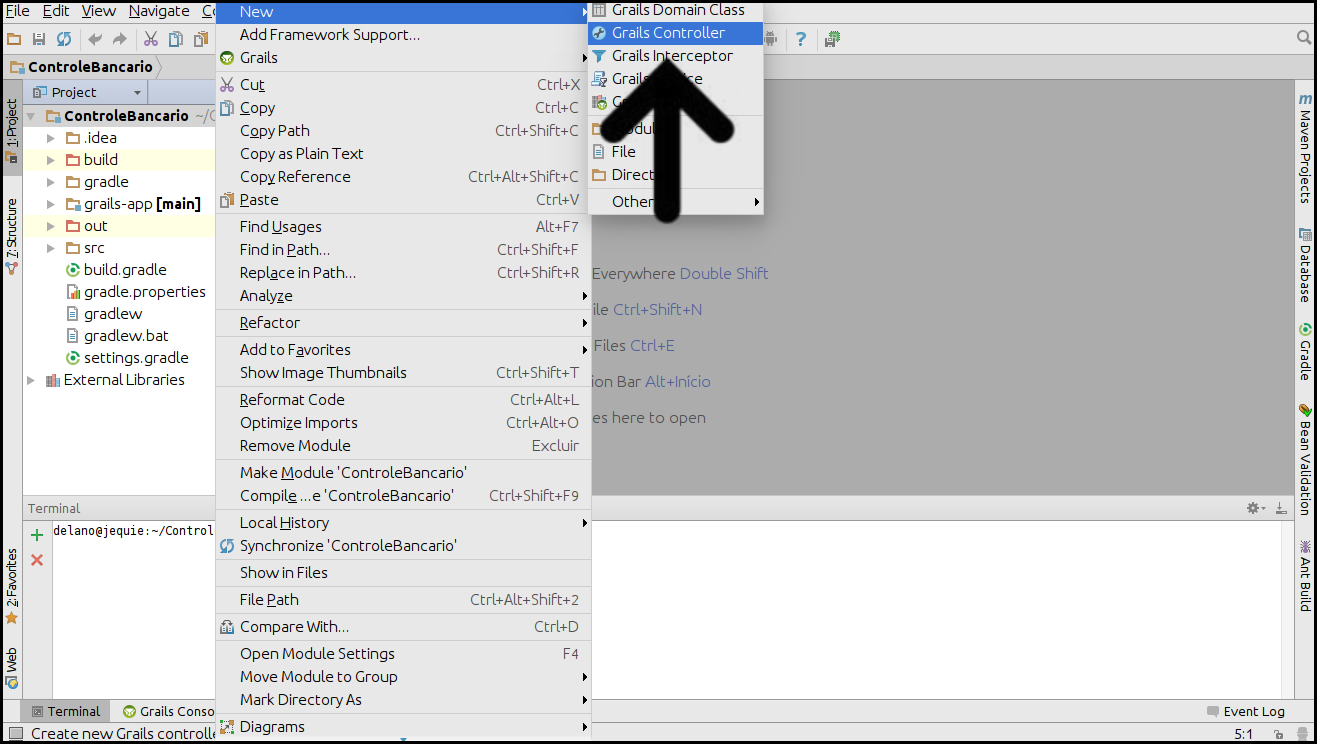
\includegraphics[width=13cm]{novoControlador}
\caption{Criação do controlador ({\it scaffolding} dinâmico).}
\label{novoControladorFig}
\end{figure}

\begin{lstlisting}[caption=Controlador {\bf TransacaoController (1)}, frame =
    trBL, float=htbp, label=codTransacaoController] 
package br.ufscar.dc.dsw

class TransacaoController {
    
    static scaffold = true

}
\end{lstlisting}

\subsection{Scaffolding Estático}\index{Scaffolding!Estático}\label{secEstatico} 

\vspace{0.5cm}

O {\it scaffolding}  estático produz, a partir de {\it  templates}, o código dos
controladores e visões que podem ser personalizados pela equipe web.  

\vspace{0.2cm}

Levando  em  consideração  esses  aspectos,  nesse  tutorial  adotou-se  o  {\it
  scaffolding} estático,  pois algumas customizações nos  controladores e visões
serão necessárias no desenvolvimento da aplicação {\bf ControleBancario}.

\begin{itemize}

\vspace{0.2cm}

\item  Para criar  um  controlador  e as  visões  (empregando {\it  scaffolding}
  estático) relacionado  à classe de  domínio {\bf Transacao}, no  IDE IntelliJ:
  Abra  o  {\bf   Terminal}  e  execute  o  comando   {\bf  grails  generate-all
    br.ufscar.dc.dsw.Transacao}. O  controlador {\bf TransacaoController.groovy}
  é criado no diretório {\bf grails-app/controllers} e o corresponde conjunto de
  {\em     Groovy     Server     Pages     (GSPs)}     no     diretório     {\bf
    grails-app/views/transacao}                       (Figura~\ref{geraTudoFig}).
  \index{Comandos!grails generate-all} 

\end{itemize}

\vspace{0.5cm}

\begin{figure}[htbp]
\centering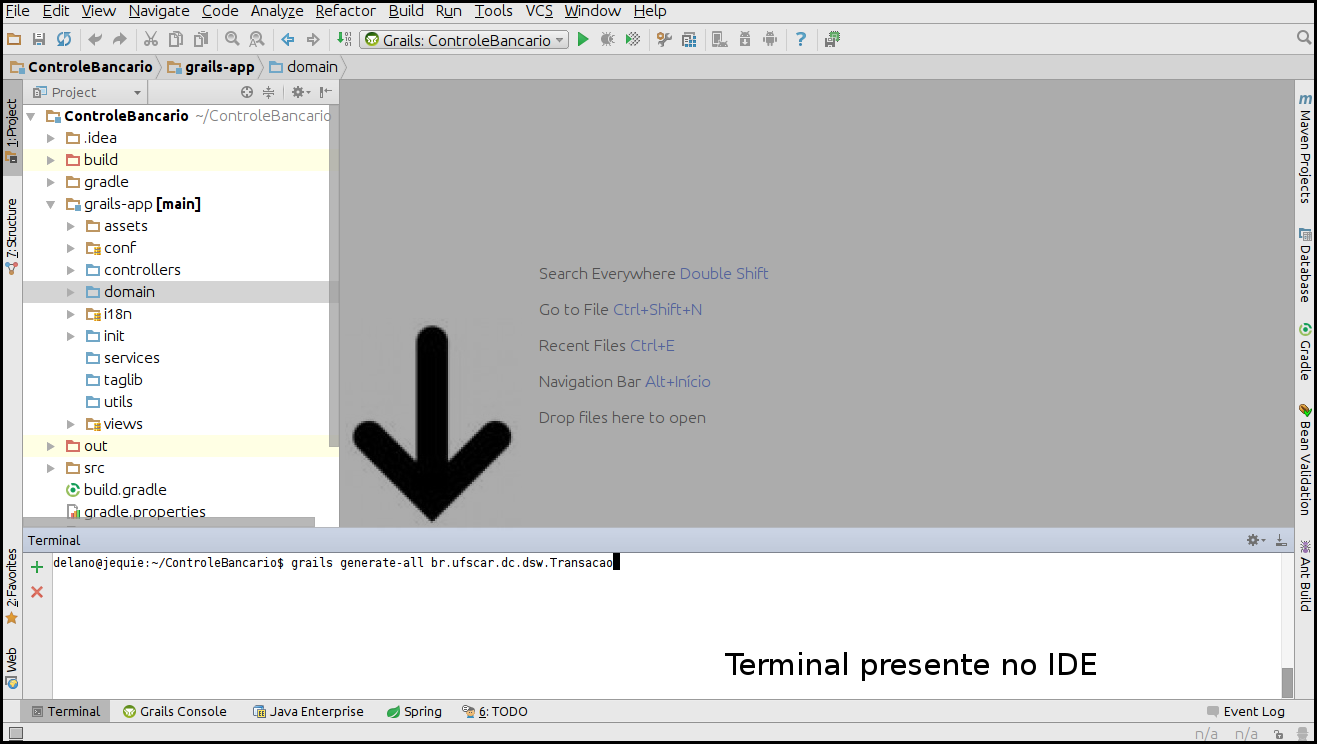
\includegraphics[width=12.5cm]{geraTudo}
\caption{Criação do controlador e das visões ({\it scaffolding} estático).}
\label{geraTudoFig}
\end{figure}

\vspace{0.5cm}

\noindent{\bf  Observação:} Para  cada método  correspondente a  uma ação  em um
controlador  é  criada  uma  correspondente  visão (arquivo  com  extensão  {\bf
  .gsp}). Por exemplo, a ação  {\bf show()} tem o correspondente {\bf show.gsp},
enquanto a ação {\bf create()} tem o correspondente {\bf create.gsp}. 

\newpage

Figura~\ref{scaffoldingFig} ilustra os controladores  e visões gerados pelo {\it
  scaffolding} da  classe de domínio {\bf Transacao}.   Destaca-se os benefícios
do paradigma {\it  Convention Over Configuration} em ação  em que nenhum arquivo
XML  é necessário para  associar esses  elementos. As  classes de  domínio estão
associadas   a   controladores  baseado   em   seus   respectivos  nomes   ({\bf
  Transacao.groovy}  $\rightarrow$ {\bf  TransacaoController.groovy}).  Conforme
já mencionado,  toda ação em um controlador  é associada a uma  visão baseada em
seu  nome ({\bf  index} $\rightarrow$  {\bf index.gsp}).   Desenvolvedores podem
configurar para  que o mapeamento seja  feito de outra maneira.   No entanto, na
maioria  das  vezes,   basta  seguir  a  convenção  e   a  aplicação  funcionará
corretamente      sem     maiores      configurações.      
\index{Convenção!{\it versus}~Configuração}

\vspace{0.5cm}

\begin{figure}[htbp]
\centering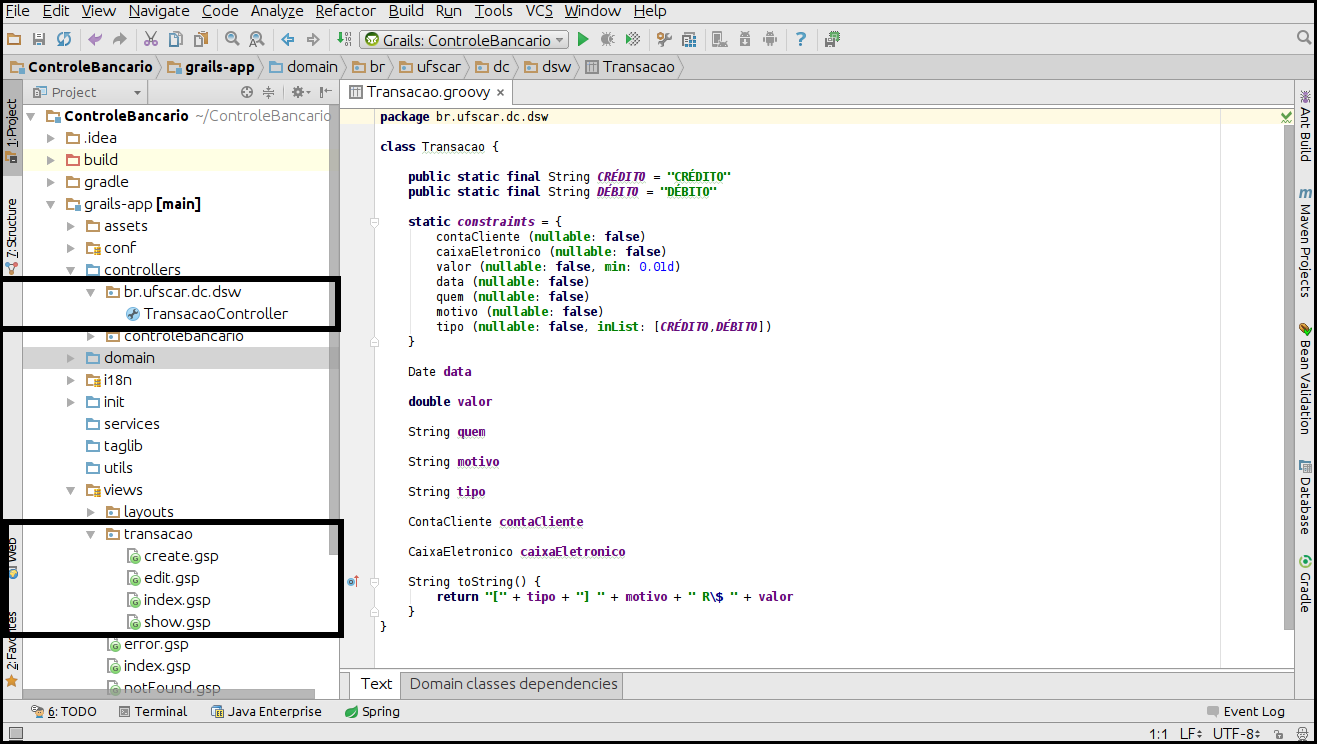
\includegraphics[width=14.5cm]{scaffolding}
\caption{Scaffolding estático das classes de domínio.}
\label{scaffoldingFig}
\end{figure}

\begin{remark}
Um bom exercício consiste em utilizar  o {\it scaffolding estático} para gerar o
controlador e as visões das demais classes de domínio.
\end{remark}

\begin{cBox}
Lembrar que não se deve gerar os  controladores e as visões para as classes {\bf
  Cliente} e {\bf Conta}.  Essas classes  são abstratas e não terão as operações
de criação, acesso, atualização e remoção (CRUD).  
\end{cBox}

\vspace{0.2cm}

\newpage

\subsection{Convenção na nomenclatura de URLs}\label{secURL}
\index{Convenção!Nomenclatura URL} 

\vspace{0.5cm}

Grails usa uma convenção (Figura~\ref{urlFig}) para automaticamente configurar o
caminho  para uma  ação em  particular. A  URL a  seguir pode  ser  entendida da
seguinte forma:

\vspace{0.5cm}

\begin{itemize}

\item ``{\it Execute a ação} {\bf show()} {\it do controlador} {\bf transacao} –
  {\it  um dos  controladores  da aplicação}  {\it  hospedada na  porta 8080  do
    servidor} {\bf localhost}''.

\end{itemize}

\begin{figure}[htbp]
\centering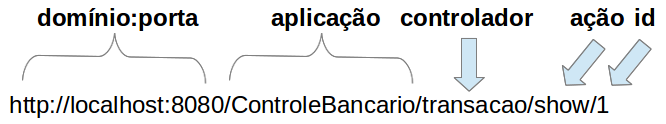
\includegraphics[width=10cm]{url}
\caption{Convenção na nomenclatura de URLs.}
\label{urlFig}
\end{figure}

A   regra  principal   de  roteamento   forma   URLs  segundo   o  padrão   {\bf
  /controlador/ação/id}, onde {\bf controlador}  é o controlador (da arquitetura
MVC) responsável  por atender  a requisição especificada  por aquela  {\it URL},
{\bf ação} é um método dentro do  controlador e {\bf id} é um parâmetro opcional
passado para identificar um objeto qualquer sobre o qual a ação será efetuada. A
visão  associada  a  essa  ação   geralmente  é  invocada  (o  controlador  pode
redirecionar para outra visão).  

\begin{cBox}
Por exemplo, {\bf /transacao/edit/1} invoca a visão {\bf transacao/edit.gsp}. 
\end{cBox}

\subsection{Controlador: TransacaoController}\label{secTransacaoController}
\index{Modelo-Visão-Controlador (MVC)!Controlador}\

\begin{lstlisting}[caption=Controlador {\bf TransacaoController},
    frame = trBL, float=htbp, label=codTransacaoController2] 
@Transactional(readOnly = true)
class TransacaoController {

    static allowedMethods = [save: "POST", update: "PUT", delete: "DELETE"]

    def index(Integer max) {
        params.max = Math.min(max ?: 10, 100)
        respond Transacao.list(params), model:[transacaoCount: Transacao.count()]
    }

    def show(Transacao transacao) {
        respond transacao
    }

    def create() {
        respond new Transacao(params)
    }

    @Transactional
    def save(Transacao transacao) {
        if (transacao == null) {
            transactionStatus.setRollbackOnly()
            notFound()
            return
        }
        if (transacao.hasErrors()) {
            transactionStatus.setRollbackOnly()
            respond transacao.errors, view:'create'
            return
        }
        transacao.save flush:true
        request.withFormat {
            form multipartForm {
                flash.message = message(code: 'default.created.message', args: [message(code: 'transacao.label', 
                                        default: 'Transacao'), transacao.id])
                redirect transacao
            }
            '*' { respond transacao, [status: CREATED] }
        }
    }

    def edit(Transacao transacao) {
        respond transacao
    }

    @Transactional
    def update(Transacao transacao) {
        if (transacao == null) {
            transactionStatus.setRollbackOnly()
            notFound()
            return
        }
        if (transacao.hasErrors()) {
            transactionStatus.setRollbackOnly()
            respond transacao.errors, view:'edit'
            return
        }
        transacao.save flush:true
        request.withFormat {
            form multipartForm {
                flash.message = message(code: 'default.updated.message', args: [message(code: 'transacao.label', 
                                        default: 'Transacao'), transacao.id])
                redirect transacao
            }
            '*'{ respond transacao, [status: OK] }
        }
    }

    @Transactional
    def delete(Transacao transacao) {

        if (transacao == null) {
            transactionStatus.setRollbackOnly()
            notFound()
            return
        }
        transacao.delete flush:true
        request.withFormat {
            form multipartForm {
                flash.message = message(code: 'default.deleted.message', args: [message(code: 'transacao.label', 
                                        default: 'Transacao'), transacao.id])
                redirect action:"index", method:"GET"
            }
            '*'{ render status: NO_CONTENT }
        }
    }

    protected void notFound() {
        request.withFormat {
            form multipartForm {
                flash.message = message(code: 'default.not.found.message', args: [message(code: 'transacao.label', 
                                        default: 'Transacao'), params.id])
                redirect action: "index", method: "GET"
            }
            '*'{ render status: NOT_FOUND }
        }
    }
}
\end{lstlisting}

Para cada classes de entidade (classe  de domínio) persistente no banco de dados
tem-se  um controlador.  Por exemplo,  durante o  {\it scaffolding}  estático, o
controlador  {\bf  TransacaoController}  foi   gerado  com  as  seguintes  ações
(Código~\ref{codTransacaoController2}):

\begin{itemize}

\vspace{0.3cm}

\item   A  ação  {\bf   index()}  é   responsável  por   retornar  a   lista  de
  instâncias. Essa lista é repassada  para visão {\bf index.gsp} que a apresenta
  em uma página HTML;

\vspace{0.3cm}

\item  A ação  {\bf  show()} é  responsável  por retornar  os  atributos de  uma
  instância.   Essa instância  é repassada  para a  visão {\bf  show.gsp}  que a
  apresenta em uma página HTML;

\vspace{0.3cm}

\item  A  ação {\bf  create()}  é  responsável por  criar  uma  instância que  é
  repassada (retornada) para a visão  {\bf create.gsp} (uma página que contém um
  formulário HTML);

\vspace{0.3cm}

\item Quando  o formulário é  submetido, a ação  {\bf save()} valida os  dados e
  caso, tenha sucesso, grava a instância  no banco de dados e redireciona para a
  ação {\bf  show()}.  Por outro  lado, se os  dados são inválidos, a  ação {\bf
    save()}  renderiza a  visão {\bf  create.gsp} novamente  para que  o usuário
  corriga os erros encontrados na validação;

\vspace{0.3cm}

\item  A ação  {\bf edit()}  é  responsável por  recuperar uma  instância a  ser
  atualizada  posteriormente.  A  instância recuperada  é  repassada (retornada)
  para a visão {\bf edit.gsp} (uma página que contém um formulário HTML);

\vspace{0.3cm}

\item Quanto o formulário é submetido  o método {\bf update()} valida os dados e
  caso, tenha sucesso, atualiza a instância no banco de dados e redireciona para
  a ação {\bf show()}.   Por outro lado, se os dados são  inválidos, a ação {\bf
    update()}  renderiza a  visão {\bf  edit.gsp} novamente  para que  o usuário
  corriga os erros encontrados na validação; e

\vspace{0.3cm}

\item Por  fim, a  ação {\bf delete()}  remove uma  instância do banco  de dados
  através  da invocação  do método  {\bf delete  (flush:true)} no  objeto  a ser
  removido.

\end{itemize}

\vspace{0.3cm}

Seguem alguns detalhes importantes:

\vspace{0.3cm}

\begin{cBox}
\begin{small}
{\bf Três  Rs:} Em Grails,  ações normalmente terminam  em uma das  três formas,
iniciadas com a letra R.

\vspace{0.3cm}
\noindent{\bf Redirecionamento}  -- a ação  solicita que o pedido  seja atendido
por uma outra ação.

\vspace{0.3cm}
\noindent{\bf Renderização}  -- envia algum conteúdo (texto  simples, XML, JSON,
HTML, etc) para ser renderizado pelo navegador.

\vspace{0.3cm}
\noindent{\bf Retorno} --  o retorno geralmente é realizado  de forma explícita.
Outras vezes  o retorno  é implícito, como  vemos no  caso de {\bf  index()} que
retorna uma lista de transações e o tamanho da lista de transações.  
\end{small}
\end{cBox}

\subsection{{\it Groovy Server Pages (GSPs)}}
\index{Modelo-Visão-Controlador (MVC)!Visão}

\vspace{0.3cm}

Durante   o   {\it  scaffolding}   estático,   as   visões  relacionadas   ({\bf
  grails-app/views/transacao})  ao controlador  {\bf  TransacaoController} foram
criadas.  Essas  visões são  {\it  Groovy Server  Pages  (GSPs)}  que podem  ser
definidas  como um  arquivo  HTML básico  que  contêm alguma  {\it tags}  Grails
(elementos {\bf <g:  ..  />}).  Para desenvolvedores Java,  as {\it tags} Grails
são semelhantes às {\it tags}  disponíveis na {\bf JavaServer Pages Standard Tag
  Libraries}
(JSTL)\footnote{\url{http://www.oracle.com/technetwork/java/index-jsp-135995.html}}

\vspace{0.2cm}

Uma característica importante de GSPs é o {\it data-binding} entre o modelo e as
variáveis acessíveis pela visão durante a renderização das páginas HTML.  Assim,
um  modelo  é um  mapa  (chave,  valor) que  a  visão  utiliza.  Por exemplo,  o
Código~\ref{codIndex} (visão  {\bf index.gsp}) tem acesso a  lista de transações
(variável   {\bf  transacaoList})   e  o   tamanho  da   lista   (variável  {\bf
  transacaoCount})   que   são   retornados   pela   ação   {\bf   index()}   --
Código~\ref{codTransacaoController2}, linha 8.  

\begin{lstlisting}[caption=Visão    {\bf    transacao/index.gsp},    frame=trBL,
    float=htbp, label=codIndex]
<!DOCTYPE html>
<html>
    <head>
        <meta name="layout" content="main" />
        <g:set var="entityName" value="${message(code: 'transacao.label', default: 'Transacao')}" />
        <title><g:message code="default.list.label" args="[entityName]" /></title>
    </head>
    <body>
        <a href="#list-transacao" class="skip" tabindex="-1"><g:message code="default.link.skip.label" default="Skip to content&hellip;"/></a>
        <div class="nav" role="navigation">
            <ul>
                <li><a class="home" href="${createLink(uri: '/')}"><g:message code="default.home.label"/></a></li>
                <li><g:link class="create" action="create"><g:message code="default.new.label" args="[entityName]" /></g:link></li>
            </ul>
        </div>
        <div id="list-transacao" class="content scaffold-list" role="main">
            <h1><g:message code="default.list.label" args="[entityName]" /></h1>
            <g:if test="${flash.message}">
                <div class="message" role="status">${flash.message}</div>
            </g:if>
            <f:table collection="${transacaoList}" />

            <div class="pagination">
                <g:paginate total="${transacaoCount ?: 0}" />
            </div>
        </div>
    </body>
</html> 
\end{lstlisting}

\noindent O  {\it data-binding}  é realizado através  da utilização da  GSP {\it
  Expression Language  (EL)} que  facilita o acesso  aos modelos através  de uma
sintaxe simples  tais como {\bf \$\{transacaoCount\}} para  uma variável simples
ou {\bf \$\{transacao.data\}} para um atributo de uma instância de objeto.

%\vspace{0.2cm}

%Seguem-se as descrições de algumas {\it tags} GSP:

%\vspace{0.2cm}

%\begin{cBox}
%\begin{itemize}

%\item A tag {\bf <g:each>} itera sobre a lista de transações, apresentando essa
%lista em uma tabela HTML. Cada  elemento da lista é armazenado na variável {\bf
%transacaoInstance}.  

%\vspace{0.2cm}

%\item   A  expressão   {\bf   \$\{fieldValue(bean:  transacaoInstance,   field:
%"valor")\}} acessa o valor do atributo {\bf valor} de cada transação presente na lista.  

%\vspace{0.2cm}

%\item     A      tag     {\bf     <g:link      action="show"     \hspace{0.2cm}
%id="\$\{transacaoInstance.id\}" \hspace{0.1cm}>} cria um {\it link} para a ação
%{\bf   show}   do   controlador    atual   (no   caso,   o   controlador   {\bf
%TransacaoController}).  
%\end{itemize}

%\end{cBox}

\section{Executando a aplicação}\index{Bootstrap}

\vspace{0.5cm}

Após gerar  o CRUD das  entidades, através do  {\it scaffolding} estático  ou do
{\it  scaffolding} dinâmico,  a aplicação  pode ser  executada. Porém,  antes de
executar a  aplicação as  instâncias das entidades  podem ser criadas.  No caso,
serão  criados  instâncias  das  entidades  ({\bf Estado},  {\bf  Cidade},  {\bf
  Endereco}, etc) na classe  {\bf BootStrap.groovy} que encontra-se no diretório
{\bf grails-app/init}. Essa classe é executada durante o {\it boot} da aplicação
e  serve, entre  outros propósitos,  para inicializar  a aplicação  por exemplo,
criando algumas instâncias de objetos.

\vspace{0.2cm}

A   implementação   da  classe   {\bf   BootStrap.groovy}   é  apresentado   nos
Códigos~\ref{codBootStrap1}~a~\ref{codBootStrap5}.   O   trecho  apresentado  no
Código~\ref{codBootStrap1}, popula  instâncias das  classes {\bf Estado}  e {\bf
  Cidade}.

\begin{lstlisting}[caption={\bf BootStrap.groovy (1)}, frame = trBL, float=htbp,
    label=codBootStrap1] 
import br.ufscar.dc.dsw.Agencia
import br.ufscar.dc.dsw.Banco
import br.ufscar.dc.dsw.CaixaEletronico
import br.ufscar.dc.dsw.Cidade
import br.ufscar.dc.dsw.Cliente
import br.ufscar.dc.dsw.ClienteFisico
import br.ufscar.dc.dsw.ClienteJuridico
import br.ufscar.dc.dsw.ContaCliente
import br.ufscar.dc.dsw.ContaCorrente
import br.ufscar.dc.dsw.ContaPoupanca
import br.ufscar.dc.dsw.Endereco
import br.ufscar.dc.dsw.Estado
import br.ufscar.dc.dsw.Gerente
import br.ufscar.dc.dsw.Transacao

class BootStrap {

    def init = { servletContext ->
       
        def sp = new Estado(sigla: 'SP', nome: 'S^ã^o Paulo')
        
        sp.save()
        if (sp.hasErrors()) {
            println sp.errors
        }
        
        println 'populando estados - ok'
        
        def sanca = new Cidade(nome: 'S^ã^o Carlos', estado: sp)
        
        sanca.save()
        if (sanca.hasErrors()) {
            println sanca.errors
        }
        
        def sampa = new Cidade(nome: 'S^ã^o Paulo', estado: sp)
        
        sampa.save()
        if (sampa.hasErrors()) {
            println sampa.errors
        }
        
        println 'populando cidades - ok'
\end{lstlisting}

\newpage

O  trecho  apresentado  no  Código~\ref{codBootStrap2},  popula  instâncias  das
classes {\bf Endereco}, {\bf Banco} e {\bf Agencia}.

\begin{lstlisting}[caption={\bf BootStrap.groovy (2)}, frame = trBL, float=htbp,
    label=codBootStrap2] 
        def end1 = new Endereco(logradouro: 'R. Conde do Pinhal', numero: 1909, 
            bairro: 'Centro', CEP: '13560-648', cidade: sanca)        
        end1.save()
        if (end1.hasErrors()) {
            println end1.errors
        }
        
        def end2 = new Endereco(logradouro: 'R. Treze de Maio', numero: 1930, 
            bairro: 'Centro', CEP: '13560-647', cidade: sanca)
        end2.save()
        if (end2.hasErrors()) {
            println end2.errors
        }
        
        def end3 = new Endereco(logradouro: 'R. Nilton Coelho de Andrade',
            numero: 772, bairro: 'Vila Maria', CEP:'03092-324', cidade: sampa)        
        end3.save()
        if (end3.hasErrors()) {
            println end3.errors
        }
        
        def end4 = new Endereco(logradouro: 'R. Humberto Manelli', numero: 50, 
            complemento: 'Apto 31', bairro: 'Jardim Gibertoni', 
            CEP:'13562-420', cidade: sanca)
        end4.save()
        if (end4.hasErrors()) {
            println end4.errors
        }
        
        println 'populando endere^ç^os - ok'

        def bb = new Banco(numero: 1, nome: 'Banco do Brasil', 
            CNPJ: '00.000.000/0001-91')
        
        bb.save()
        if (bb.hasErrors()) {
            println bb.errors
        }
        
        def santander = new Banco(numero: 33, nome: 'Santander', 
            CNPJ: '90.400.888/0001-42')
        
        santander.save()
        if (santander.hasErrors()) {
            println santander.errors
        }

        println 'populando bancos - ok'
        
        def agencia1 = new Agencia(numero: 1888, nome: 'Conde do Pinhal', 
            endereco: end1, banco: bb)
        
        agencia1.save()
        if (agencia1.hasErrors()) {
            println agencia1.errors
        }
        
        def agencia2 = new Agencia(numero: 24, nome: 'Treze de Maio', 
            endereco: end2, banco: santander)
        
        agencia2.save()
        if (agencia2.hasErrors()) {
            println agencia2.errors
        }
        
        println 'populando ag^ê^ncias - ok'
\end{lstlisting}

\newpage

\hyphenation{CaixaEletronico}

O  trecho  apresentado  no  Código~\ref{codBootStrap3},  popula  instâncias  das
classes  {\bf  Gerente},  {\bf  CaixaEletronico},  {\bf  ClienteFisico}  e  {\bf
  ClienteJuridico}. 

\begin{lstlisting}[caption={\bf BootStrap.groovy (3)}, frame = trBL, float=htbp,
    label=codBootStrap3]
        def gerente1 = new Gerente(nome: 'Carlos da Silva', rg: '1234 SSP/SP',
            CPF: '129.304.458-07', agencia: agencia1
        )
    
        gerente1.save()
        if (gerente1.hasErrors()) {
            println gerente1.errors
        }
        
        def gerente2 = new Gerente(nome: 'Maria Jos^é^', rg: '3467 SSP/RJ',
            CPF: '018.990.444-50', agencia: agencia2
        )
    
        gerente2.save()
        if (gerente2.hasErrors()) {
            println gerente2.errors
        }
        
        println 'populando gerentes - ok'
        
        def caixa1 = new CaixaEletronico(banco: bb, endereco: end1)
        
        caixa1.save()
        if (caixa1.hasErrors()) {
            println agencia1.errors
        }
        
        def caixa2 = new CaixaEletronico(banco: santander, endereco: end2)
        
        caixa2.save()
        if (caixa2.hasErrors()) {
            println agencia1.errors
        }
        
        println 'populando caixas eletr^ô^nicos - ok'
        
        def cliFisico = new ClienteFisico(nome: 'Fulano de Tal', 
            rg: '13567 SSP/SP', CPF: '018.990.444-50', endereco: end4,
            dtMoradia: new Date(), status: Cliente.ATIVO) 
        
        cliFisico.save()
        if (cliFisico.hasErrors()) {
            println cliFisico.errors
        }
        
        println 'populando clientes f^í^sicos - ok'
                
        def cliJuridico = new ClienteJuridico(nome: 'Via^çã^o Cometa S/A', 
            CNPJ: '61.084.018/0001-03', endereco: end3,
            dtMoradia: new Date(), status: Cliente.ATIVO) 
        
        cliJuridico.save()
        if (cliJuridico.hasErrors()) {
            println cliJuridico.errors
        }
        
        println 'populando clientes jur^í^dicos - ok'
\end{lstlisting}

\newpage

\hyphenation{ContaPoupanca}
\hyphenation{Transacao}

O  trecho  apresentado  no  Código~\ref{codBootStrap4},  popula  instâncias  das
classes  {\bf ContaCorrente},  {\bf ContaPoupanca}  e {\bf  Transacao}. Conforme
pode-se observar,  as instâncias da  classe {\bf Transacao}  criadas representam
depósitos e saques.
  
\begin{lstlisting}[caption={\bf BootStrap.groovy (4)}, frame = trBL, float=htbp,
    label=codBootStrap4]
        def corrente = new ContaCorrente(agencia: agencia1, 
            numero: '010414688', saldo: 1000.56d, limite: 500.00d,
            abertura: new Date()
        )
    
        corrente.save()
        if (corrente.hasErrors()) {
            println corrente.errors
        }

        def contaCli1 = new ContaCliente(conta: corrente, 
            cliente: cliJuridico, titular: true
        )
    
        contaCli1.save()
        if (contaCli1.hasErrors()) {
            println contaCli1.errors
        }
        
        println 'populando contas correntes (associado ao cliente jur^í^dico) - ok'
                
        def poupanca = new ContaPoupanca(agencia: agencia2, 
            numero: '261327', saldo: 10000.56d, juros: 0.50d,
            correcao: 1.20d, dia: 23, abertura: new Date()
        )
    
        poupanca.save()
        if (poupanca.hasErrors()) {
            println poupanca.errors
        }

        def contaCli2 = new ContaCliente(conta: poupanca, 
            cliente: cliFisico, titular: true
        )
    
        contaCli2.save()
        if (contaCli2.hasErrors()) {
            println contaCli2.errors
        }
        
        println 'populando contas poupan^ç^as (associado ao cliente f^í^sico) - ok'
        
	def deposito = new Transacao(contaCliente: contaCli2, caixaEletronico: caixa2, 
            valor: 50d, data: new Date(), quem: 'Pr^ó^prio', motivo: 'Dep^ó^sito',
            tipo: Transacao.CR^É^DITO
        )
        
        deposito.save()
        if (deposito.hasErrors()) {
            println deposito.errors
        }
        
        println 'populando depositos - ok'
        
        def saque = new Transacao(contaCliente: contaCli1, caixaEletronico: caixa1, 
            valor: 100d, data: new Date(), quem: 'Pr^ó^prio', motivo: 'Saque', 
            tipo: Transacao.D^É^BITO)
        
        saque.save()
        if (saque.hasErrors()) {
            println saque.errors
        }
        
        println 'populando saques - ok'
\end{lstlisting}

\newpage

E por fim, o trecho apresentado no Código~\ref{codBootStrap5}, popula instâncias
da classe  {\bf Transacao}. Conforme  pode-se observar, as instâncias  da classe
{\bf Transacao} criadas representam transferências bancárias.

\begin{lstlisting}[caption={\bf BootStrap.groovy (5)}, frame = trBL, float=htbp,
    label=codBootStrap5] 
        def transf1 = new Transacao(contaCliente: contaCli1, 
            caixaEletronico: caixa2, valor: 25d, data: new Date(),
            quem: 'Pr^ó^prio', motivo: 'Transfer^ê^ncia', tipo: Transacao.D^É^BITO)
        
        def transf2 = new Transacao(contaCliente: contaCli2, 
            caixaEletronico: caixa2, valor: 25d, data: new Date(),
            quem: 'Fulano de Tal', motivo: 'Transfer^ê^ncia', 
            tipo: Transacao.CR^É^DITO)
        
        transf1.save()
        if (transf1.hasErrors()) {
            println transf1.errors
        }
        
        transf2.save()
        if (transf2.hasErrors()) {
            println transf2.errors
        }
        
        println 'populando transfer^ê^ncias - ok'
    }

    def destroy = {
    }
}
\end{lstlisting}

\vspace{0.3cm}

Para executar a  aplicação, clique no botão direito do mouse  no ícone {\bf Run:
  Grails} (Figura~\ref{executarFig}).  A aplicação é implantada no servidor {\it
  Web},   como   pode    ser   observado   na   janela   {\bf    Run}   do   IDE
IntelliJ. \index{Comandos!grails run-app} 
\vspace{0.3cm}

\begin{itemize}

\item     A     aplicação    pode     ser     acessada     através    da     URL
  {\footnotesize\url{http://localhost:8080}}.    Se   o   navegador  não   abrir
  automaticamente, cole a  URL em um navegador e a  aplicação será acessada.  Os
  controladores da aplicação serão listados (Figura~\ref{executarFig}).  
\end{itemize}

\vspace{0.2cm}

\begin{figure}[htbp]
\centering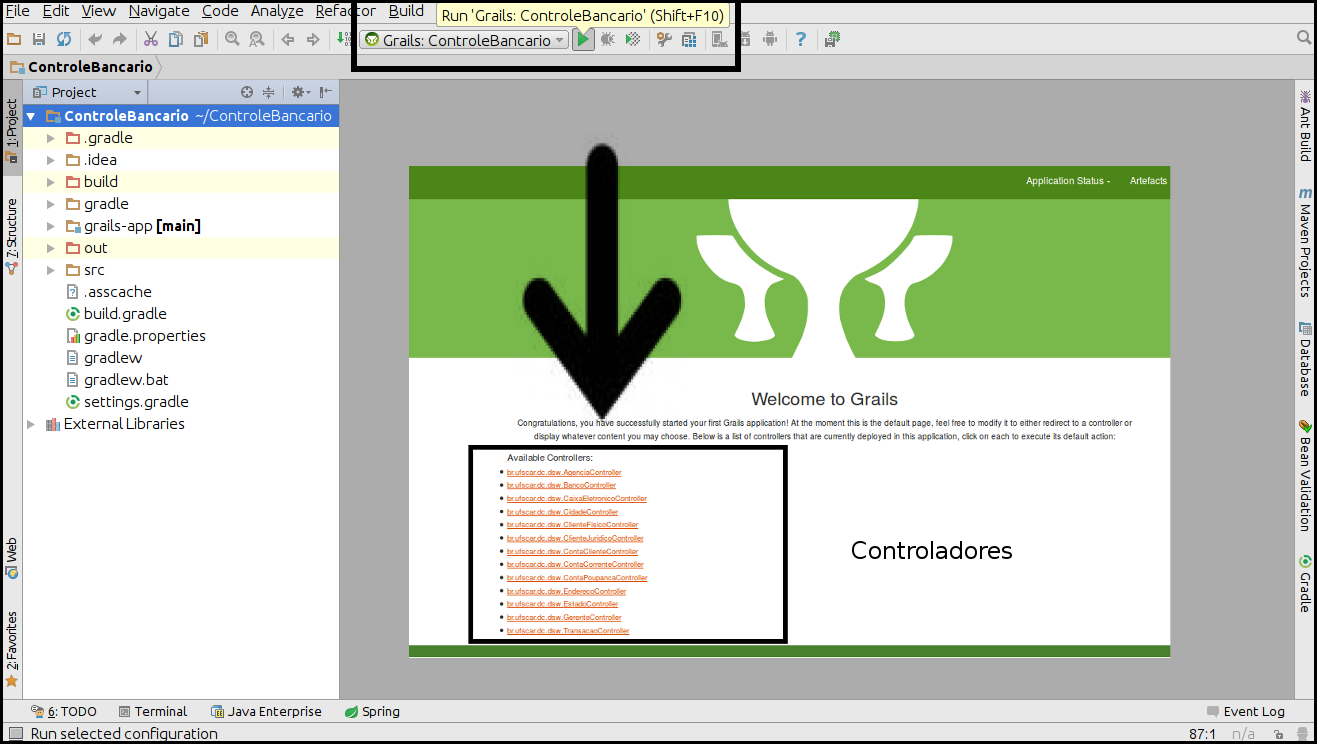
\includegraphics[width=14cm]{runApp}
\caption{Execução da aplicação {\bf ControleBancario}}
\label{executarFig}
\end{figure}

\vspace{0.3cm}

\begin{itemize}

\item   Ao  clicar  no   link  {\bf   br.ufscar.dc.dsw.TransacaoController},  as
  transações  bancárias  inseridas  anteriormente ({\bf  BootStrap.groovy})  são
  apresentadas (Figura~\ref{listaTransacoesFig}). 

\end{itemize}

\vspace{0.5cm}

\begin{figure}[htbp]
\centering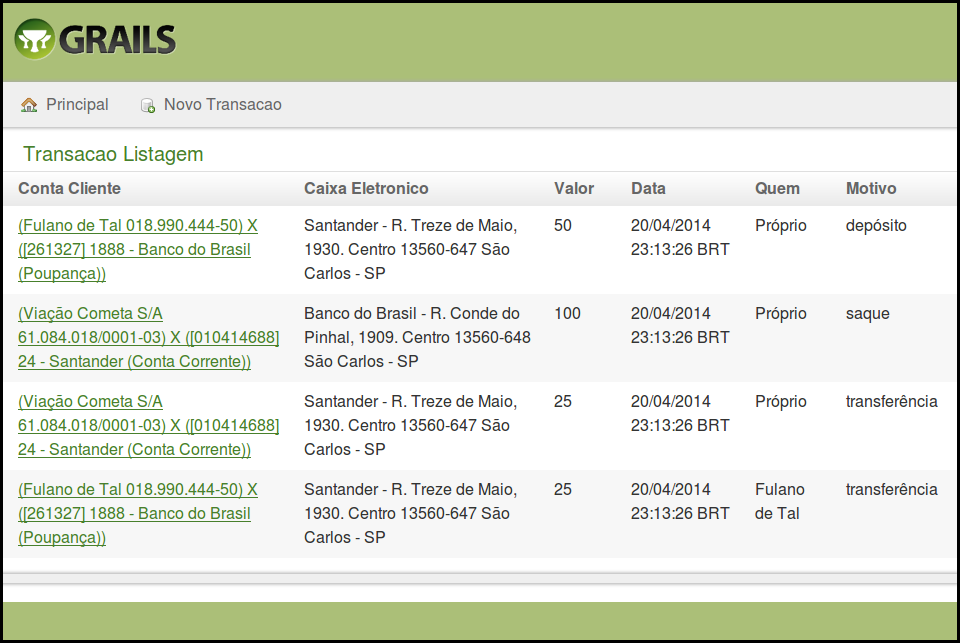
\includegraphics[width=13cm]{listaTransacoes}
\caption{Lista de transações bancárias}
\label{listaTransacoesFig}
\end{figure}

\vspace{0.5cm}

\begin{itemize}

\item Clique em {\bf Novo Transacao}  e crie uma nova transação bancária. Quando
  clicar em {\bf Criar}, observe que você poderá {\bf Editar} ou {\bf Remover} a
  transação. Por  fim, ao clicar em  {\bf Transacao Listagem}, a  nova entrada é
  apresentada na lista de transações (Figura~\ref{novaTransacaoFig}). 

\end{itemize}

\vspace{1cm}

\begin{figure}[htbp]
\centering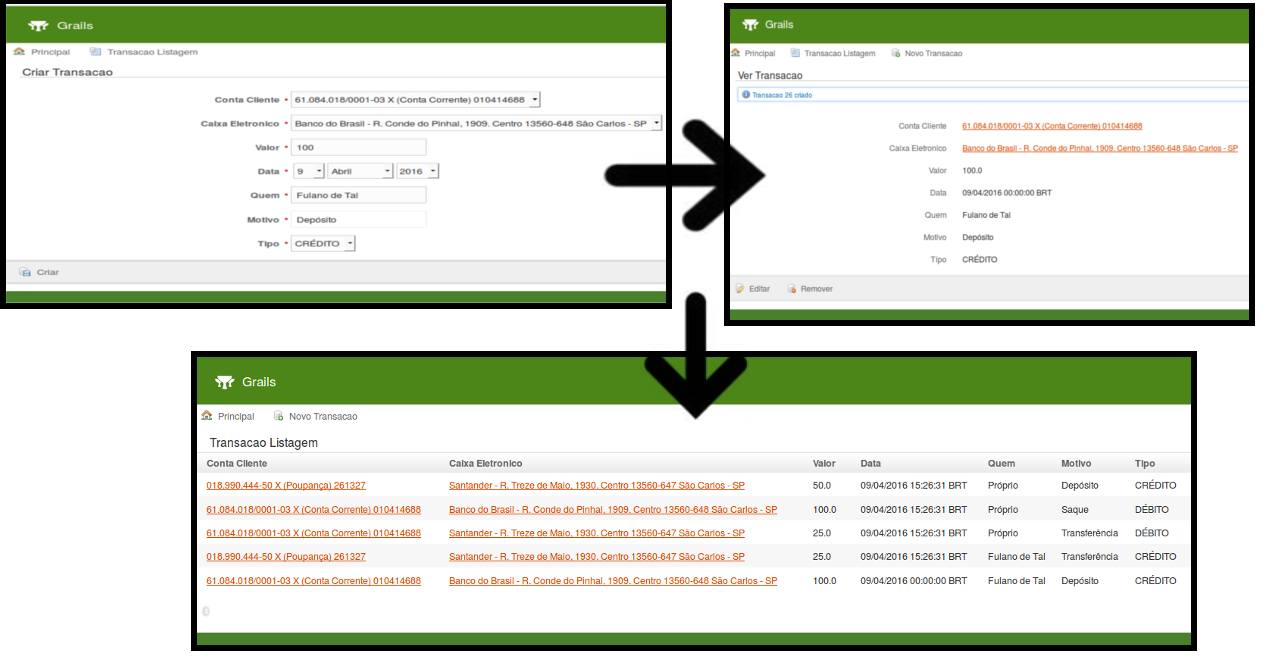
\includegraphics[width=13cm]{novaTransacao}
\caption{Criação de uma nova transação bancária}
\label{novaTransacaoFig}
\end{figure}

\vspace{0.5cm}

Salienta-se que para a criação das outras entidades da aplicação ({\bf Cliente},
{\bf Conta} e outros), os passos são análogos.  

\newpage

\begin{itemize}

\item Clique  em {\bf  Novo Transacao}  e crie uma  nova transação  bancária com
  valores  inválidos   (Figura~\ref{transacaoInvalidaFig}).   Verfica-se  que  a
  transação não foi criada, pois as validações de dados foram violadas. 

\end{itemize}

\begin{figure}[htbp]
\centering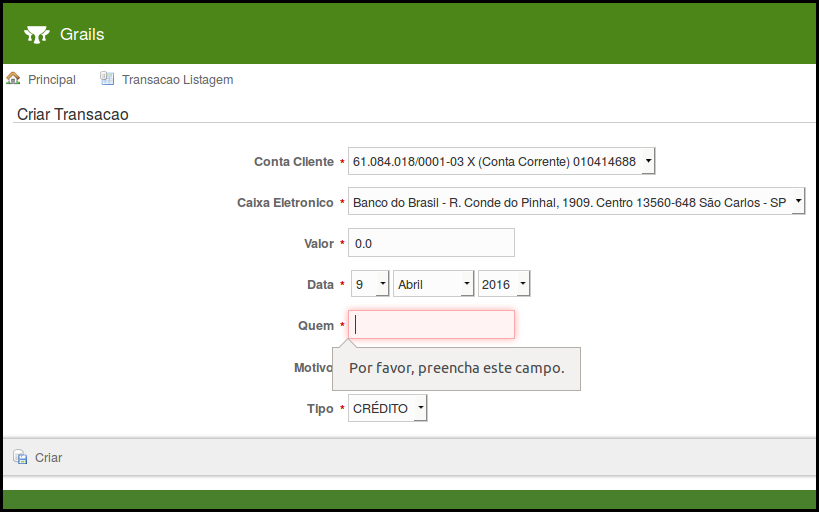
\includegraphics[width=12cm]{transacaoInvalida}
\caption{Criação de uma transação bancária com valores inválidos}
\label{transacaoInvalidaFig}
\end{figure}

\vspace{0.5cm}

\begin{remark}
Sugere-se, como aprendizado, executar os  demais controladores e verificar se as
demais funcionalidades da aplicação encontram-se funcionando corretamente.
\end{remark}

\section{Considerações finais}

\vspace{0.3cm}

Esse   capítulo  apresentou   uma  implementação   parcial  da   aplicação  {\bf
  ControleBancario}.         O        código-fonte        dessa        aplicação
({\footnotesize\texttt{ControleBancarioV1}})   encontra-se   disponível  em   um
repositório                      {\it                      GitHub}\footnote{URL:
  {\url{https://github.com/delanobeder/FG}}}.  

\vspace{0.2cm}

Dando continuidade ao desenvolvimento em Grails, o próximo capítulo apresenta a
implementação   de  novas   funcionalidades  no   contexto  da   aplicação  {\bf
  ControleBancario}.  


